% ----------------------------------------------------------
% Apêndices
% Documentos gerados pelo próprio autor
% ----------------------------------------------------------

% ---
% Inicia os apêndices
% ---
\begin{apendicesenv}

% Imprime uma página indicando o início dos apêndices
\partapendices
\chapter{Protótipo}
\label{apendice-prototipo}

Este apêndice apresenta um registro dos protótipos de alta fidelidade desenhados para o projeto.

Na Figura \ref{prototipoLandingPage} é apresentado o protótipo da 1º parte da tela de Landing Page.

\begin{figure}[H]
	\centering
	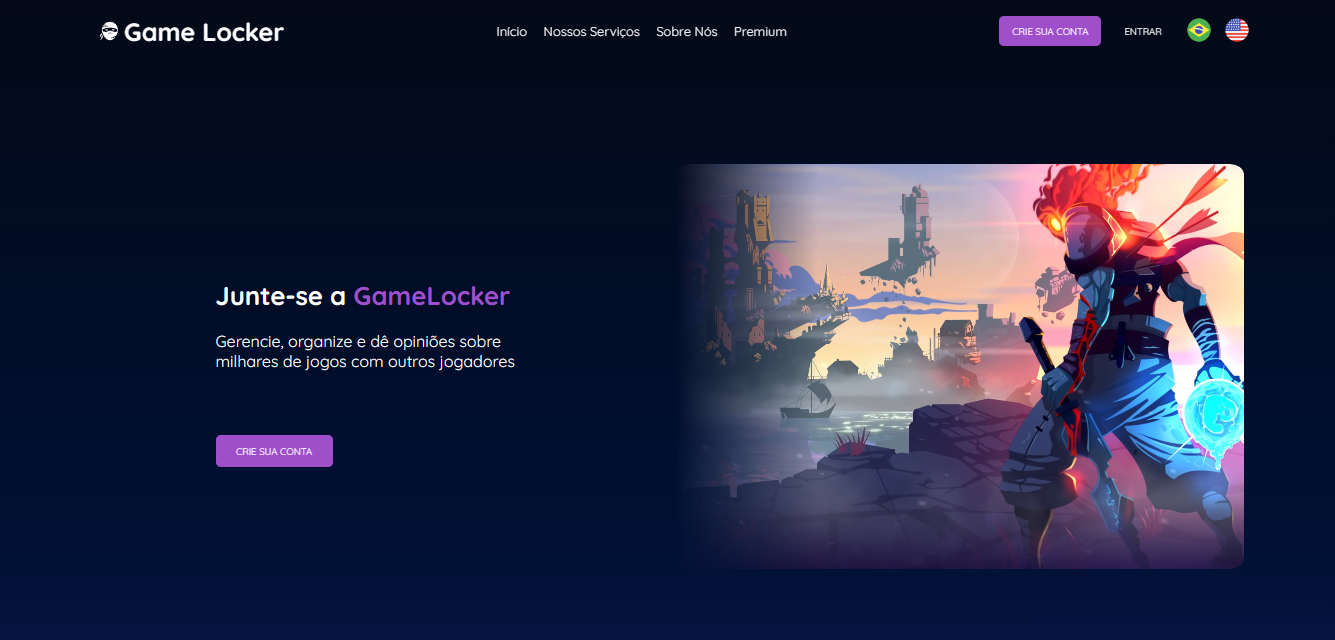
\includegraphics[width=1\textwidth,keepaspectratio]{./imagens/PrototipoLandingPage.png}
	\caption{Protótipo Landing Page 1}
	Fonte: Os autores
    \label{prototipoLandingPage}
\end{figure}
\pagebreak

Na Figura \ref{prototipoLandingPage2} é apresentado o protótipo da 2º parte da tela de Landing Page.

\begin{figure}[H]
	\centering
	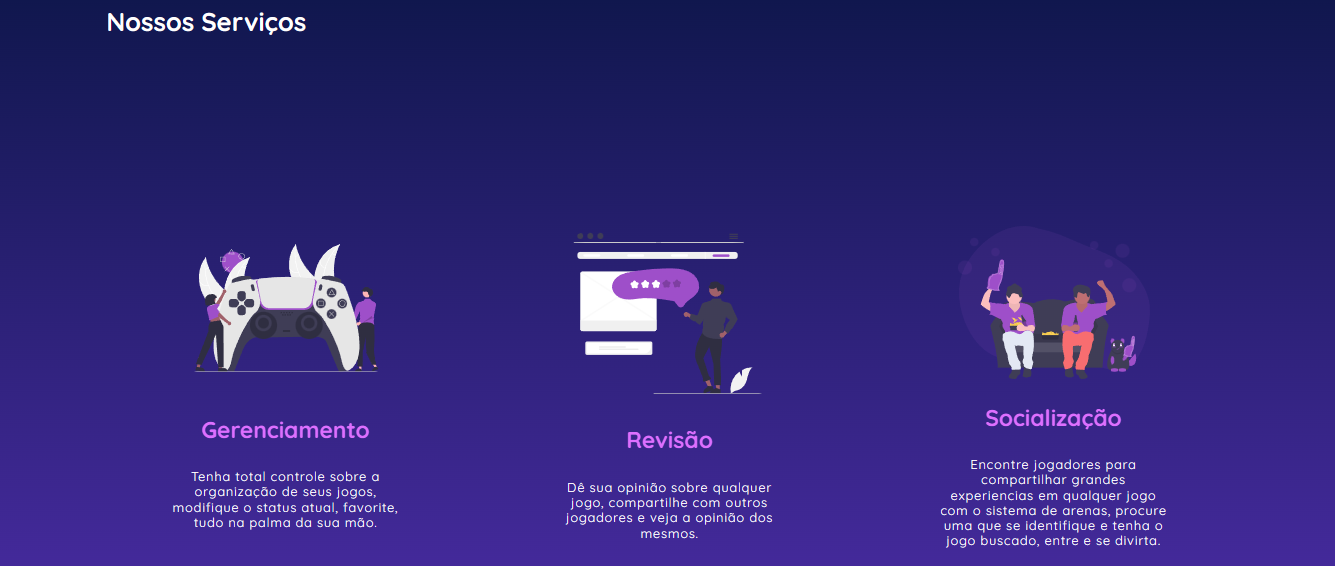
\includegraphics[width=1\textwidth,keepaspectratio]{./imagens/PrototipoLandingPage2.png}
	\caption{Protótipo Landing Page 2}
	Fonte: Os autores
    \label{prototipoLandingPage2}
\end{figure}

Na Figura \ref{prototipoLandingPage3} é apresentado o protótipo da 3º parte da tela de Landing Page.

\begin{figure}[H]
	\centering
	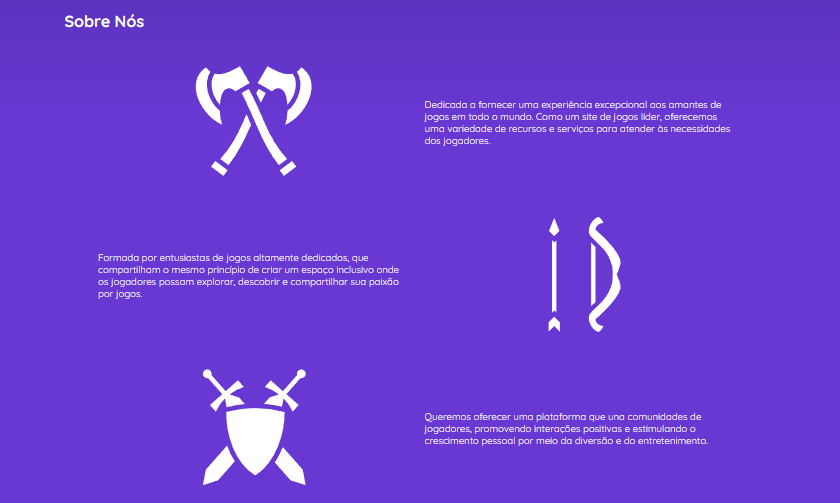
\includegraphics[width=1\textwidth,keepaspectratio]{./imagens/PrototipoLandingPage3.png}
	\caption{Protótipo Landing Page 3}
	Fonte: Os autores
    \label{prototipoLandingPage3}
\end{figure}
\pagebreak

Na Figura \ref{prototipoLandingPage4} é apresentado o protótipo da 4º parte da tela de Landing Page.

\begin{figure}[H]
	\centering
	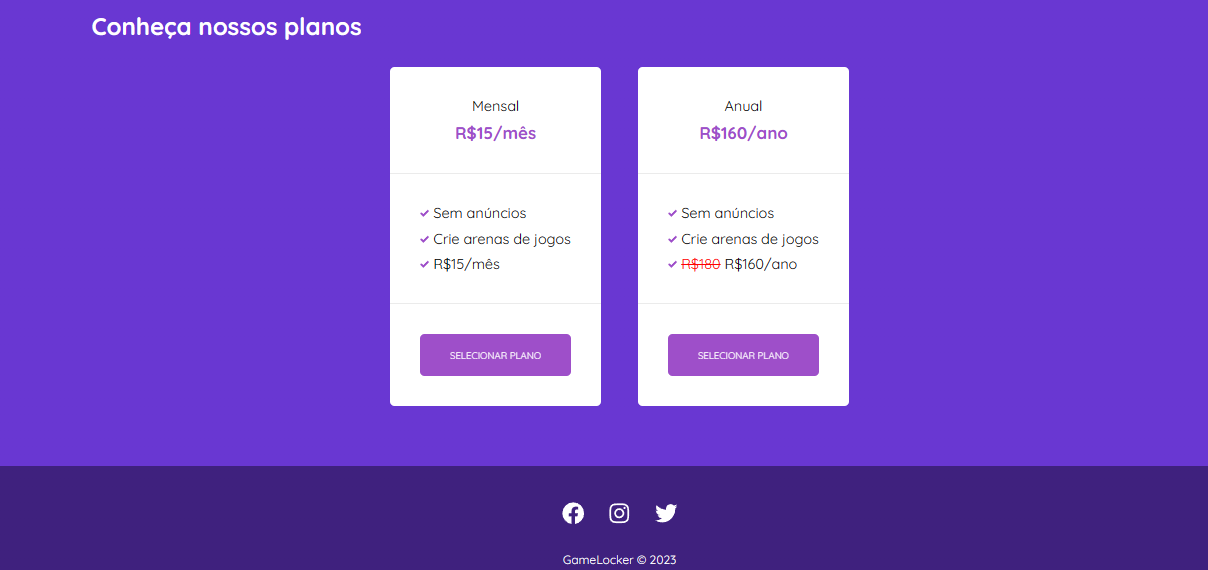
\includegraphics[width=1\textwidth,keepaspectratio]{./imagens/PrototipoLandingPage4.png}
	\caption{Protótipo Landing Page 4}
	Fonte: Os autores
    \label{prototipoLandingPage4}
\end{figure}

Na Figura \ref{prototipoCadastro} é apresentado o protótipo da tela de Cadastro.

\begin{figure}[H]
	\centering
	
\includegraphics[width=1\textwidth,keepaspectratio]{./imagens/PrototipoCadastro.png}
	\caption{Protótipo Cadastro}
	Fonte: Os autores
    \label{prototipoCadastro}
\end{figure}
\pagebreak

Na Figura \ref{prototipoLogin} é apresentado o protótipo da tela de Login.

\begin{figure}[H]
	\centering
	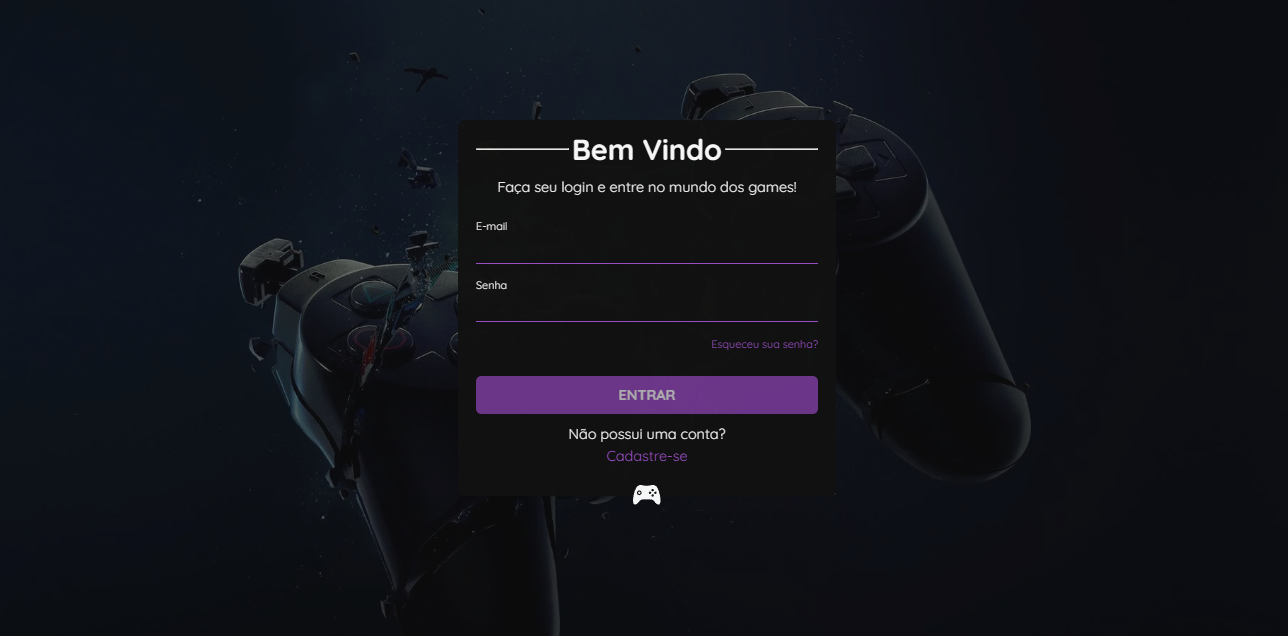
\includegraphics[width=1\textwidth,keepaspectratio]{./imagens/PrototipoLogin.png}
	\caption{Protótipo Login}
	Fonte: Os autores
    \label{prototipoLogin}
\end{figure}

Na Figura \ref{prototipoPortal} é apresentado o protótipo da 1º parte da tela do Portal.

\begin{figure}[H]
	\centering
	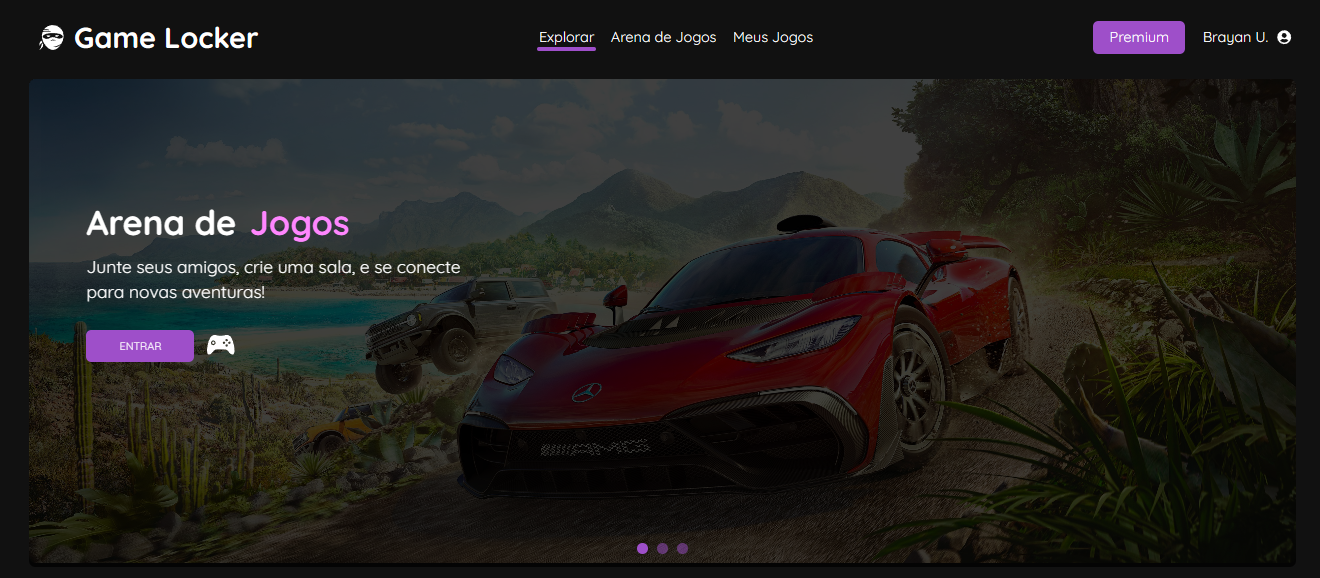
\includegraphics[width=1\textwidth,keepaspectratio]{./imagens/PrototipoPortal.png}
	\caption{Protótipo Portal 1}
	Fonte: Os autores
 \label{prototipoPortal}
\end{figure}
\pagebreak

Na Figura \ref{prototipoPortal2} é apresentado o protótipo da 2º parte da tela do Portal.

\begin{figure}[H]
	\centering
	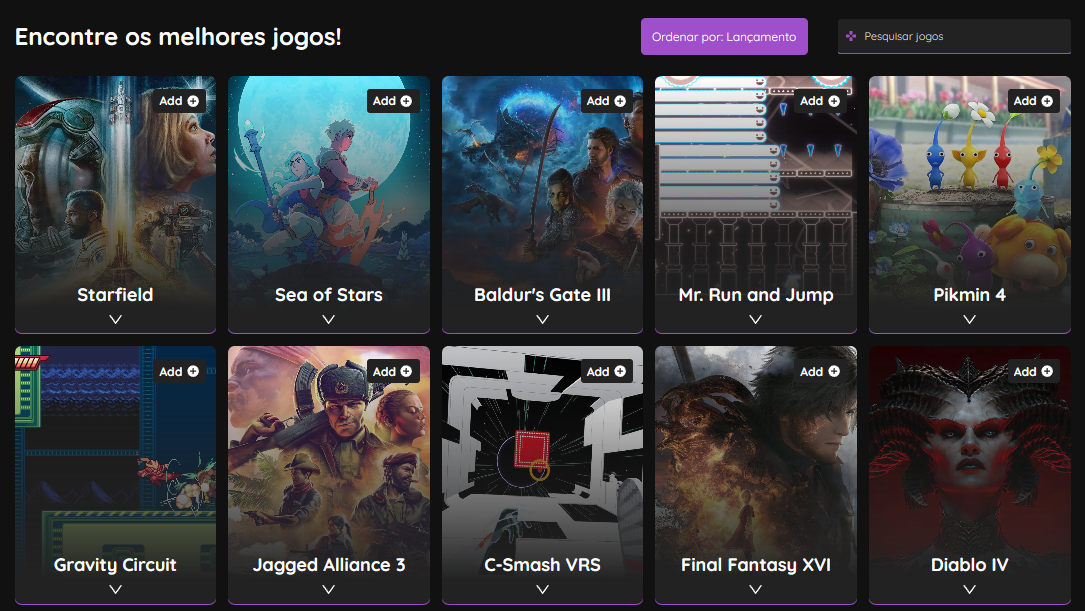
\includegraphics[width=1\textwidth,keepaspectratio]{./imagens/PrototipoPortal2.png}
	\caption{Protótipo Portal 2}
	Fonte: Os autores
 \label{prototipoPortal2}
\end{figure}
\pagebreak

Na Figura \ref{prototipoPortal3} é apresentado o protótipo da 3º parte da tela do Portal.

\begin{figure}[H]
	\centering
	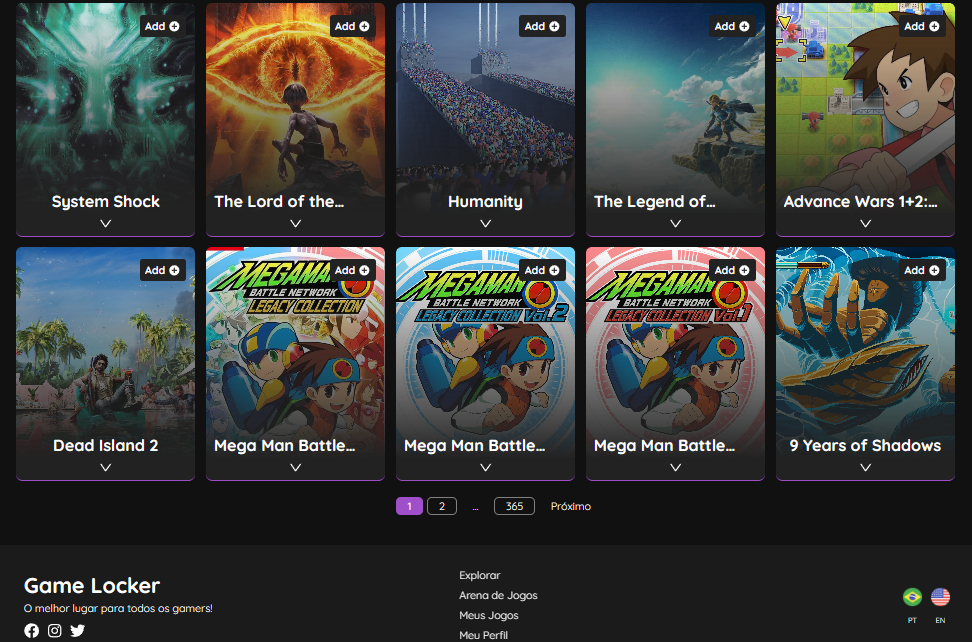
\includegraphics[width=1\textwidth,keepaspectratio]{./imagens/PrototipoPortal3.png}
	\caption{Protótipo Portal 3}
	Fonte: Os autores
 \label{prototipoPortal3}
\end{figure}
\pagebreak

Na Figura \ref{prototipoReview} é apresentado o protótipo do modal de Review.

\begin{figure}[H]
	\centering
	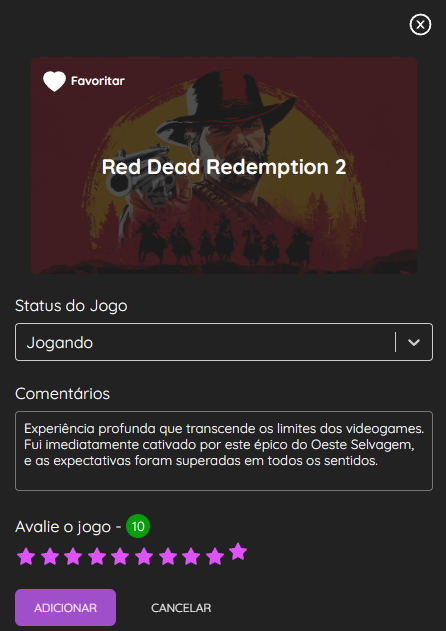
\includegraphics[scale=0.7]{./imagens/PrototipoReview.png}
	\caption{Protótipo Review}
	Fonte: Os autores
    \label{prototipoReview}
\end{figure}
\pagebreak

Na Figura \ref{prototipoMeuPerfil} é apresentado o protótipo da tela do Meu Perfil.

\begin{figure}[H]
	\centering
	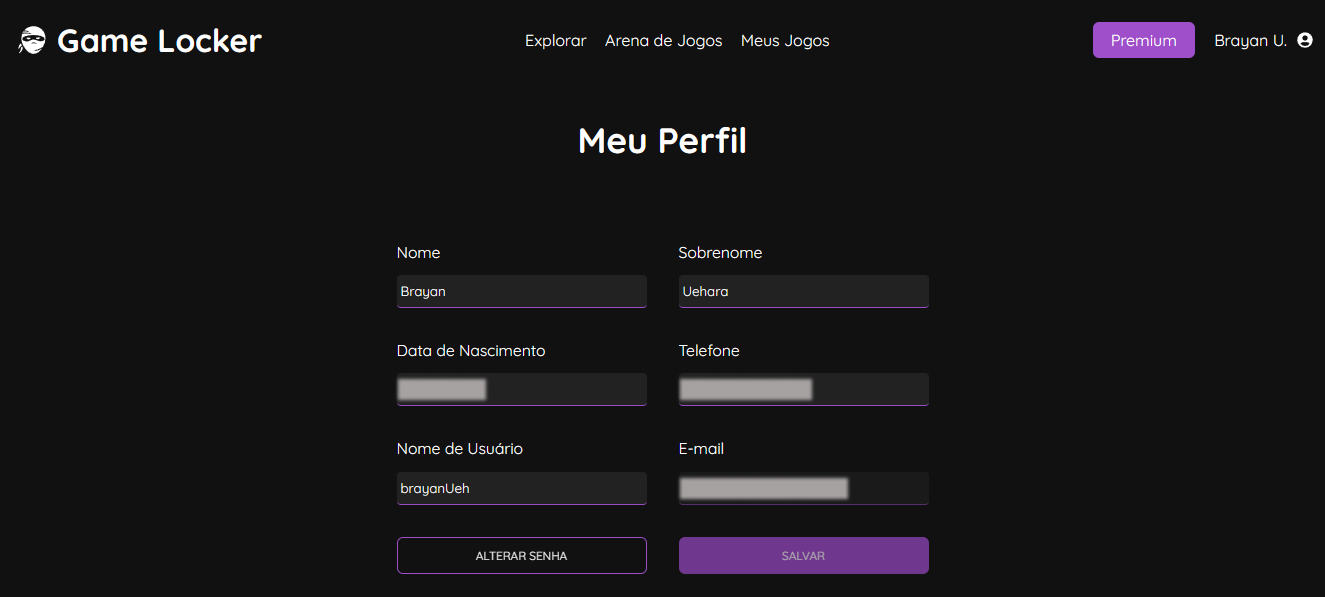
\includegraphics[scale=0.34]{./imagens/PrototipoMeuPerfil.png}
	\caption{Protótipo Meu Perfil}
	Fonte: Os autores
    \label{prototipoMeuPerfil}
\end{figure}

Na Figura \ref{prototipoMeuJogos} é apresentado o protótipo da tela do Meu Jogos.

\begin{figure}[H]
	\centering
	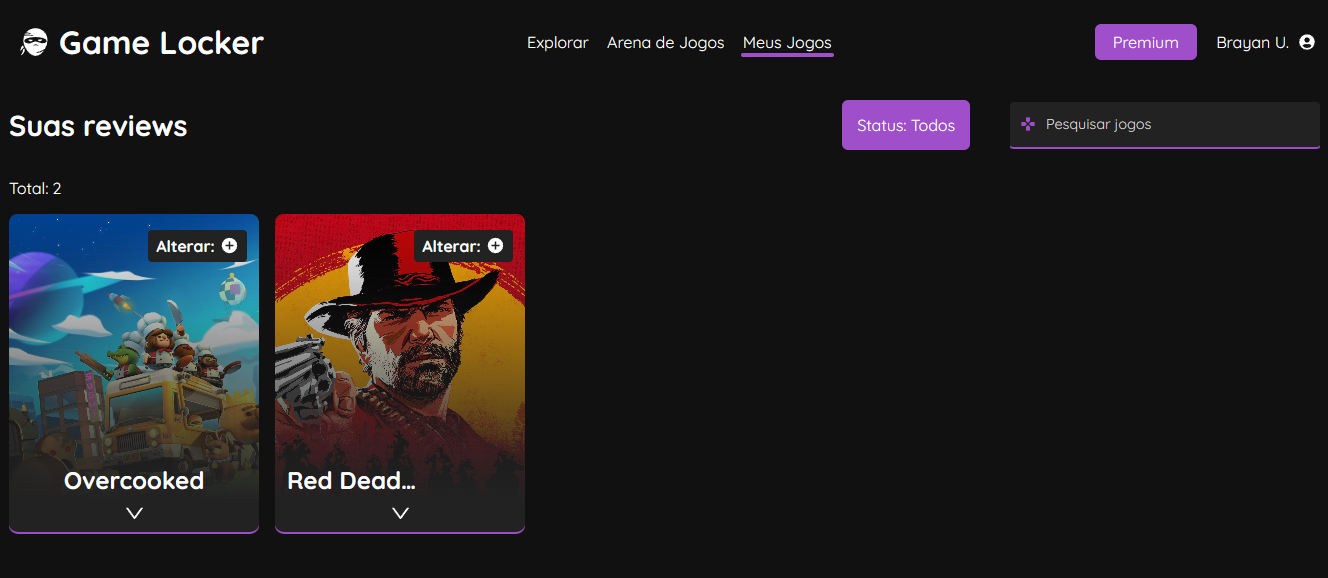
\includegraphics[scale=0.45]{./imagens/PrototipoMeuJogos.png}
	\caption{Protótipo Meu Jogos}
	Fonte: Os autores
    \label{prototipoMeuJogos}
\end{figure}
\pagebreak

Na Figura \ref{prototipoPagamento} é apresentado o protótipo da tela de Pagamento.

\begin{figure}[H]
	\centering
	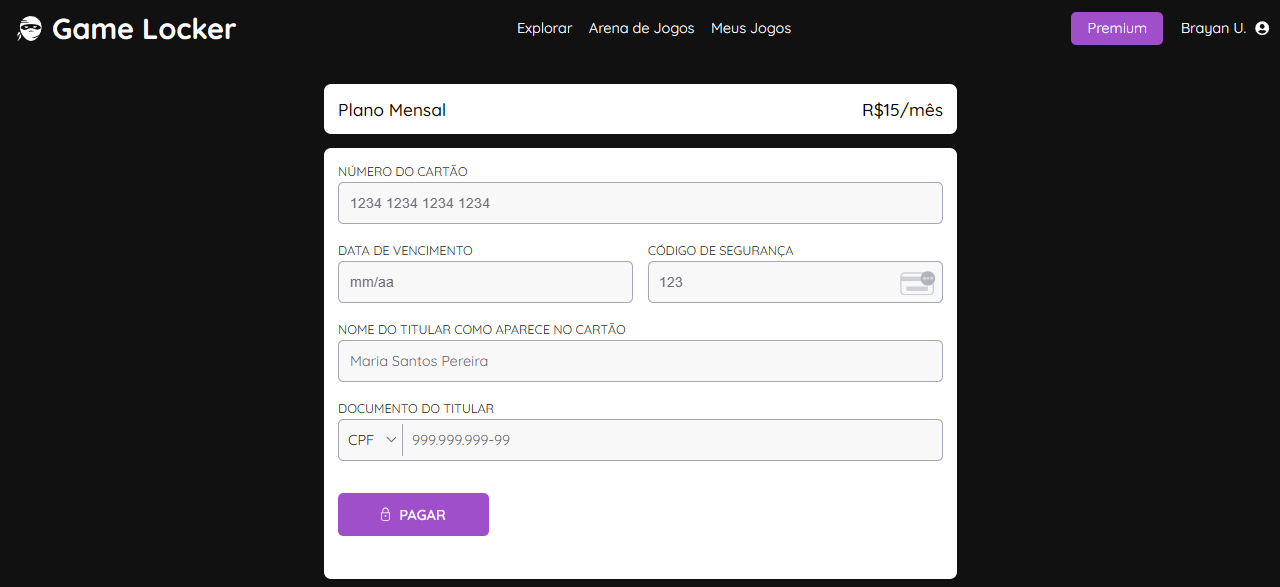
\includegraphics[scale=0.45]{./imagens/PrototipoPagamento.png}
	\caption{Protótipo Pagamento}
	Fonte: Os autores
    \label{prototipoPagamento}
\end{figure}
\pagebreak

Na Figura \ref{prototipoArena} é apresentado o protótipo da 1º parte da tela da Arena.

\begin{figure}[H]
	\centering
	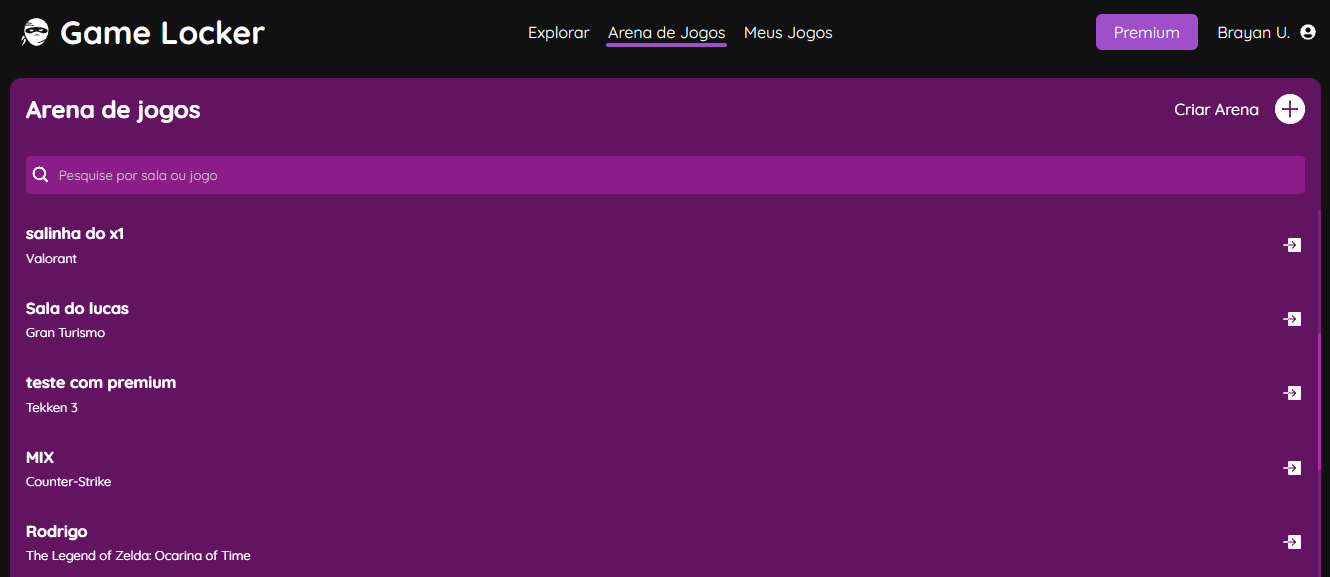
\includegraphics[scale=0.45]{./imagens/PrototipoArena.png}
	\caption{Protótipo Arena}
	Fonte: Os autores
    \label{prototipoArena}
\end{figure}

Na Figura \ref{prototipoArena2} é apresentado o protótipo da 2º parte da tela da Arena.

\begin{figure}[H]
	\centering
	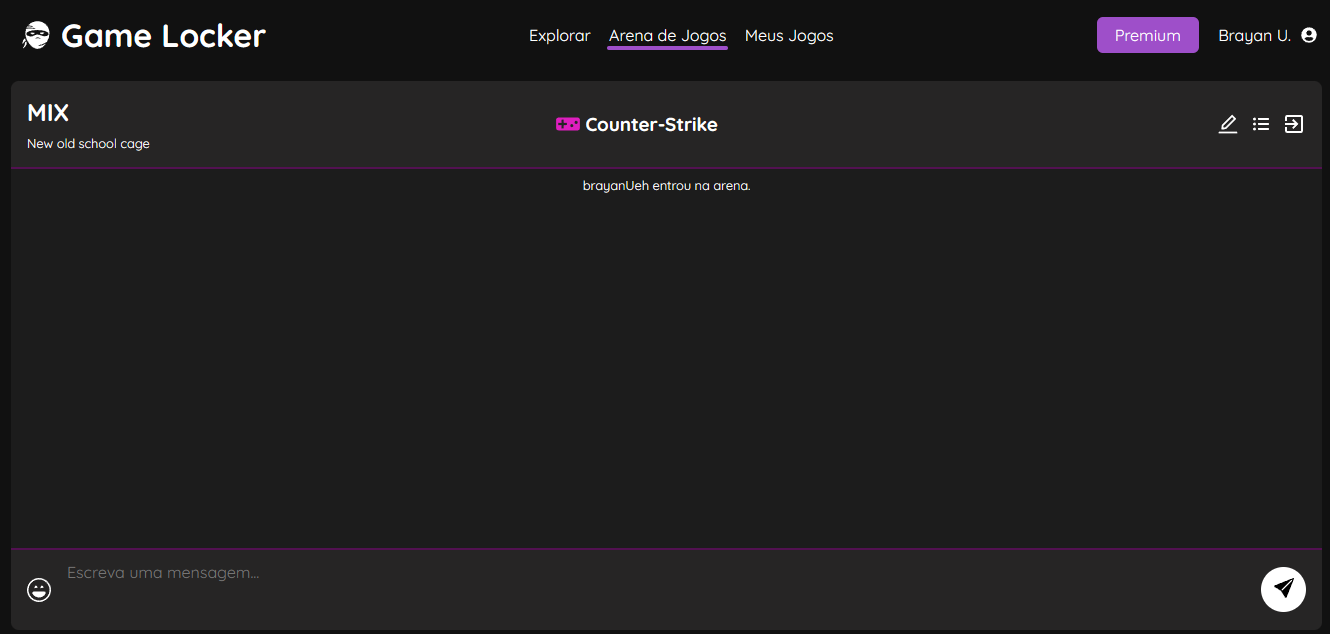
\includegraphics[scale=0.45]{./imagens/PrototipoArena2.png}
	\caption{Protótipo Arena 2}
	Fonte: Os autores
    \label{prototipoArena2}
\end{figure}
\pagebreak

Na Figura \ref{prototipoEncontrarAmigos} é apresentado o protótipo da 1º parte da tela de Encontrar Amigos.

\begin{figure}[H]
	\centering
	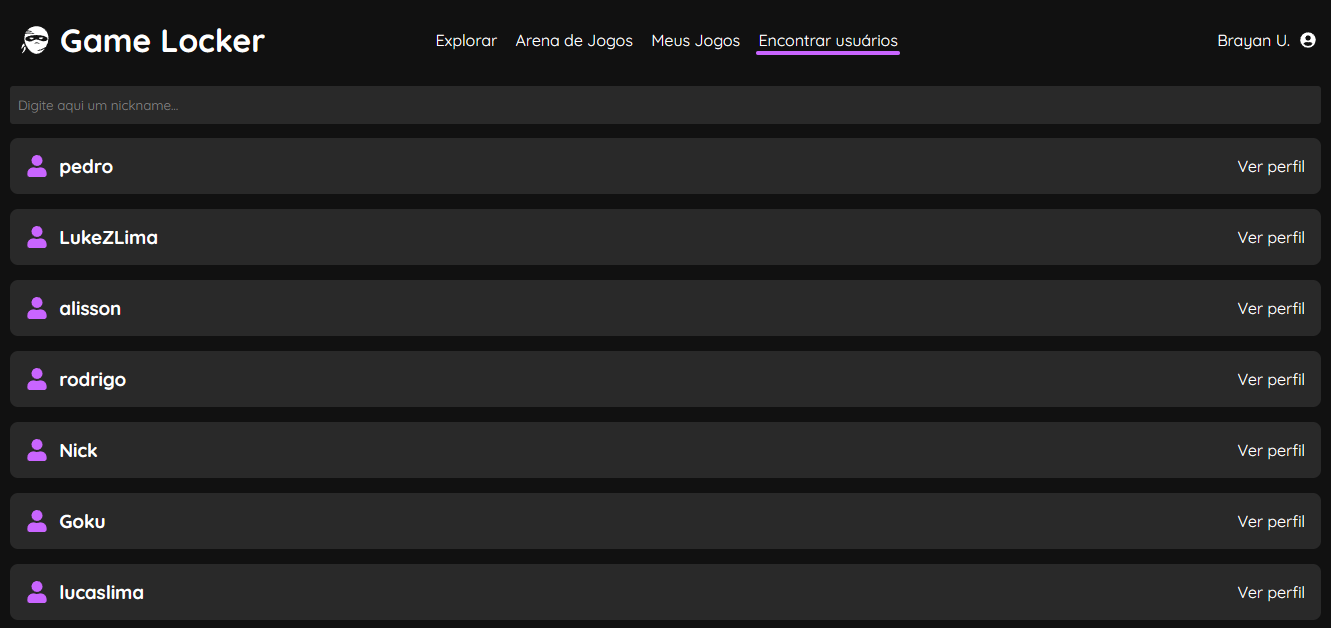
\includegraphics[scale=0.45]{./imagens/PrototipoEncontrarAmigos.png}
	\caption{Protótipo Encontrar Amigos}
	Fonte: Os autores
    \label{prototipoEncontrarAmigos}
\end{figure}

Na Figura \ref{prototipoEncontrarAmigos2} é apresentado o protótipo da 2º parte da tela de Encontrar Amigos

\begin{figure}[H]
	\centering
	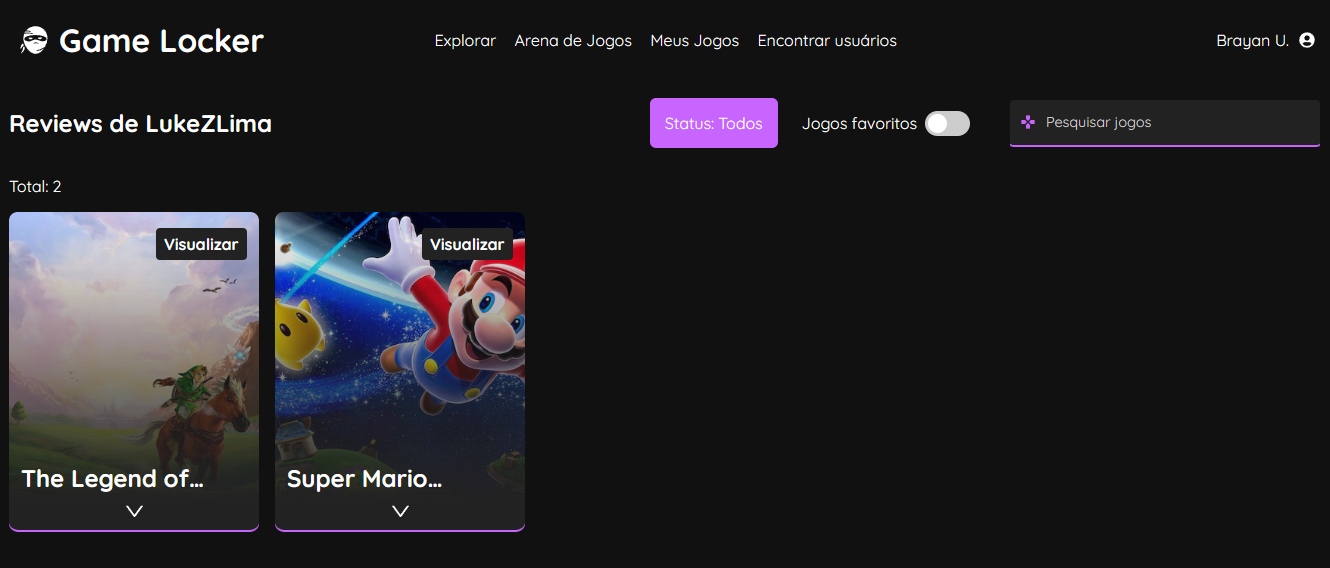
\includegraphics[scale=0.45]{./imagens/PrototipoEncontrarAmigos2.png}
	\caption{Protótipo Encontrar Amigos 2}
	Fonte: Os autores
    \label{prototipoEncontrarAmigos2}
\end{figure}
\pagebreak

\chapter{Reuniões}
\label{ata-reunião}

\section{Reunião 1 - (04/03/2023)}
Com as equipes criadas, foram elencados principais pontos a se pensar:

\begin{itemize}
    \item Dias de Reunião
    \item Tema principal
    \item Tecnologias a serem utilizadas
    \item Funções básicas de cada membro
\end{itemize}

\section{Reunião 2 - (11/03/2023)}
Após a definição do tema do projeto, iniciou-se o processo de concepção, incluindo a criação de um protótipo de baixa fidelidade, considerando as funcionalidades a serem implementadas, o layout e, simultaneamente, preparou-se uma apresentação inicial.

Após uma análise minuciosa, a equipe optou por adotar o Kanban como metodologia de gerenciamento, visando assegurar um fluxo eficiente e organizado no desenvolvimento do projeto. Além disso, foram realizados preparativos para abranger as atividades requeridas, incluindo a criação de um canal no \textit{\gls{Youtube}}, e a implementação de controle de versão utilizando SVN, entre outras práticas necessárias.

\section{Reunião 3 - (18/03/2023)}
Foi realizada uma discussão detalhada para explicitar as funções de cada membro da equipe, buscando uma organização clara e eficiente. Além disso, a documentação foi aprimorada com base nos \textit{feedbacks} recebidos, visando uma execução do projeto que atendesse às expectativas de ambas as partes envolvidas, resultando em um trabalho no qual todos estivessem satisfeitos.

\section{Reunião 4 - (25/03/2023)}
A equipe dedicou seu esforço à estruturação do projeto, dividindo as responsabilidades entre as áreas de \textit{\gls{Front-end}}, \textit{\gls{Back-end}} e Banco de Dados. O foco principal foi estabelecer uma comunicação eficiente entre essas áreas, garantindo uma integração harmoniosa. 

Com as funções de cada membro claramente definidas durante a reunião anterior, o desenvolvimento foi iniciado de maneira simplificada. Simultaneamente, a equipe realizou outras atividades requisitadas, garantindo uma abordagem multitarefa para maximizar a eficiência do projeto.

\section{Reunião 5 - (01/04/2023)}
Nesta reunião, a equipe concentrou-se no desenvolvimento do desenho do projeto, o que incluiu a criação da arquitetura a ser utilizada, o Modelo Entidade-Relacionamento (MER) e o Diagrama Entidade-Relacionamento (DER). Foi dedicado tempo para planejar e visualizar a estrutura do sistema, mapeando as relações entre as entidades e definindo a organização dos dados. Simultaneamente, a equipe manteve-se atualizada com todas as outras dependências requisitadas, garantindo que o projeto estivesse alinhado com todas as exigências e expectativas estabelecidas.

\section{Reunião 6 - (08/04/2023)}
Nesta reunião, a equipe se dedicou a discutir os \textit{feedbacks} recebidos sobre a documentação, analisando as sugestões fornecidas e identificando as melhores abordagens para aprimorá-la. Durante essa análise, foram discutidas maneiras de evoluir a documentação, incorporando as sugestões relevantes e garantindo que estivesse completa e precisa.

Além disso, a equipe trabalhou na criação da identidade do projeto, deliberando sobre um nome definitivo, desenvolvendo logos e selecionando as cores que seriam utilizadas. Concomitantemente, atendendo à solicitação, a equipe iniciou o processo de criação do desenho da aplicação. Esse passo foi crucial para preparar uma apresentação futura, possibilitando uma visualização clara e detalhada do layout da aplicação que seria desenvolvida.

\section{Reunião 7 - (15/04/2023)}
Nesta reunião, os pontos destacados na documentação foram cuidadosamente abordados e resolvidos, garantindo que a documentação estivesse completa, precisa e atendesse aos padrões exigidos. Além disso, o desenvolvimento do Desenho da Aplicação continuou, com a equipe se esforçando para aprimorá-lo com base nos \textit{feedbacks} recebidos durante as aulas e ao tirar dúvidas.

Paralelamente, a equipe prosseguiu com a criação do projeto, incluindo o desenvolvimento da API que seria utilizada como parte do \textit{\gls{Back-end}} do sistema. Ao mesmo tempo, o \textit{\gls{Front-end}} da aplicação também estava sendo elaborado, permitindo uma visão mais clara e tangível do objetivo do projeto. 

\section{Reunião 8 - (22/04/2023)}
Após a conclusão do Desenho da Aplicação, a equipe deu início ao desenvolvimento da Prova de Conceito (POC). Durante esse período, houve um esforço contínuo para aprimorar a documentação, revisar e melhorar as arquiteturas estabelecidas e incorporar ideias provenientes tanto dos \textit{feedbacks} fornecidos pelo professor quanto das discussões entre os próprios membros da equipe.

\section{Reunião 9 - (29/04/2023)}
Nesta reunião, a equipe dedicou-se a uma análise detalhada da Prova de Conceito (POC), com o objetivo de identificar e corrigir qualquer erro ou problema existente. A revisão minuciosa visava minimizar o maior número de erros possível antes de considerar a POC como finalizada e pronta para entrega.

\section{Reunião 10 - (06/05/2023)}
Com a conclusão da Prova de Conceito (POC), a equipe deu início ao desenvolvimento do MVP (Mínimo Produto Viável) do projeto. Durante essa fase, houve um esforço conjunto para trabalhar na documentação, garantindo que estivesse atualizada e refletisse com precisão as últimas decisões e modificações feitas no projeto. Simultaneamente, foi elaborada uma lista inicial de funcionalidades que deveriam ser incluídas no MVP.

\begin{itemize}
    \item Funcionalidade de cadastro.
    \item Guardar Sessão de Login 
    \item Adicionar Reviews 
    \item Visualizar, editar e remover reviews.
    \item Filtragem de jogos no portal.
\end{itemize}

\section{Reunião 11 - (13/05/2023)}
A equipe começou a documentar a API utilizando a ferramenta Swagger, o que proporcionou uma documentação mais clara e organizada para os leitores. O Swagger é uma ferramenta poderosa que permite descrever, consumir e visualizar APIs de forma interativa. Isso não apenas facilitou a compreensão da API para os desenvolvedores, mas também proporcionou uma maneira eficiente de explorar e testar os \textit{\gls{Endpoints}} da API.

Além disso, a equipe continuou o desenvolvimento do código, implementando funcionalidades adicionais e fazendo melhorias contínuas na documentação à medida que novos requisitos e desafios eram descobertos durante o processo de desenvolvimento.

\section{Reunião 12 - (20/05/2023)}
Nesta reunião, a equipe concentrou-se em aprimorar todas as documentações já entregues e nas que ainda seriam entregues, visando fornecer uma base sólida e compreensível para o desenvolvimento do MVP (Mínimo Produto Viável). Durante o encontro, foram revisados detalhadamente os documentos existentes, buscando melhorar a clareza, precisão e abrangência das informações apresentadas.

\section{Reunião 13 - (27/05/2023)}
Na reunião realizada, o foco principal foi discutir o andamento atual do projeto. A equipe dedicou-se a identificar possíveis falhas ou pontos fracos no desenvolvimento até o momento. O objetivo era identificar áreas que precisavam de melhorias, correções ou otimizações.

\section{Reunião 14 - (03/06/2023)}
Durante a reunião, a equipe finalizou os slides para a Apresentação Final, realizando revisões por todos os membros para garantir que o conteúdo estivesse coerente com o que foi requisitado. Cada detalhe foi cuidadosamente analisado para assegurar clareza e precisão nas informações apresentadas.

Além disso, foi dado um foco especial ao \textit{\gls{Front-end}} do projeto. Todas as funcionalidades necessárias foram revisadas para garantir que estivessem implementadas corretamente e apresentadas de forma clara e intuitiva para os usuários. A interface do usuário foi refinada para proporcionar uma experiência fluida e agradável, priorizando a usabilidade e a compreensão das funcionalidades.

\section{Reunião 15 - (10/06/2023)}
Na reunião desta semana, nossa equipe compartilhou os detalhes de duas atividades cruciais em que estivemos focados recentemente. Primeiramente, discutimos os ajustes no Deploy do Back-end da aplicação, descrevendo à otimização e aprimoramento da infraestrutura de hospedagem do sistema. 

Durante a reunião, enfatizamos nosso compromisso em garantir que a apresentação seja clara, concisa e impactante, destacando os pontos fortes do MVP e seu potencial para agregar valor aos usuários finais, \textit{stakeholders} e parceiros envolvidos no projeto.

\section{Reunião 16 - (31/07/2023)}
Na reunião desta semana, dedicamos nosso tempo à integração dos novos membros da equipe, realizando uma sessão especial para delineação das responsabilidades individuais de cada membro. Durante o encontro, conduzimos discussões detalhadas sobre as pendências do projeto, analisando cuidadosamente cada tarefa que ainda estava por ser concluída.

Com base nessas informações essenciais, colaboramos ativamente para elaborar um cronograma estruturado e detalhado que servirá como guia durante a construção do projeto. 

\section{Reunião 17 - (07/08/2023)}
Na reunião desta semana, nossa equipe concentrou-se em dois aspectos-chave do projeto: o aprimoramento do estudo financeiro e a conclusão da funcionalidade de confirmação de e-mail. Durante o encontro, realizamos uma análise detalhada do estudo financeiro, examinando todos os elementos financeiros do empreendimento. Discutimos o orçamento, identificamos áreas potenciais para economia e otimização de gastos e projetamos custos futuros.

Além disso, celebramos o sucesso da equipe na implementação da funcionalidade de confirmação de e-mail em nossa aplicação. Essa reunião foi fundamental para garantir que todos na equipe estivessem alinhados com as metas financeiras do projeto e cientes dos avanços técnicos realizados.

\section{Reunião 18 - (14/08/2023)}
Na reunião da semana, nossa equipe de projeto realizou uma sessão altamente produtiva, concentrando-se em duas frentes essenciais: o desenvolvimento das principais funcionalidades da aplicação e a preparação do ambiente para o \textit{Google AdSense}.

O encontro foi marcado por discussões detalhadas e decisões cruciais. Iniciamos com uma análise cuidadosa das ferramentas e tecnologias necessárias para criar a Arena de Jogos. Simultaneamente, dedicamos uma parte significativa da reunião à preparação do ambiente para o \textit{Google AdSense}. 

\section{Reunião 19 - (21/08/2023)}
Na reunião realizada, nossa equipe de projeto seguiu um plano estruturado, focando em duas frentes cruciais para o progresso do projeto. Primeiramente, dedicamos uma parte significativa do tempo à revisão e aprimoramento detalhado da documentação do projeto. 

Simultaneamente, nos dedicamos ao aprofundamento do entendimento do sistema de pagamento. Realizamos uma análise dos requisitos técnicos, exploramos as ferramentas utilizadas no sistema, avaliamos cuidadosamente as considerações de segurança e absorvemos as melhores práticas relacionadas.

\section{Reunião 20 - (28/08/2023)}
Na reunião, nossa equipe focou seus esforços em duas áreas vitais do projeto. Primeiramente, dedicamos tempo ao aprimoramento da interface e dos \textit{\gls{Endpoints}} da Arena de Jogos. Discutimos melhorias específicas para garantir uma experiência de usuário mais intuitiva e eficaz. Cada membro da equipe compartilhou suas ideias e sugestões para enriquecer a navegação na plataforma.

Simultaneamente, investimos parte da reunião na pesquisa e avaliação de alternativas para a incorporação de anúncios em nosso sistema. Discutimos os obstáculos encontrados e começamos a considerar outras opções criativas para a monetização do projeto.

\section{Reunião 21 - (04/09/2023)}
Durante a reunião planejada, nossa equipe elaborou um plano estratégico abrangente para impulsionar o desenvolvimento da Arena de Jogos. Definimos claramente nossos objetivos, priorizando a implementação bem-sucedida do recurso de chat e os pequenos detalhes que precisavam ser resolvidos e delineamos um cronograma para a implementação do \textit{webhook}. Além disso, dedicamos uma parte significativa da reunião ao aprimoramento do processo de redefinição de senha. 

\section{Reunião 22 - (11/09/2023)}
Na reunião, iniciamos com um marco importante: a implementação do \textit{Webhook} na Arena de Jogos. Esse progresso significativo não apenas visa aprimorar a experiência dos jogadores, mas também elevar a funcionalidade da arena, permitindo uma comunicação mais eficiente e interativa entre os participantes, tornando-a ainda mais envolvente e dinâmica para os jogadores. Além disso, discutimos detalhadamente e confirmamos nossa estratégica decisão de adotar a API do Mercado Pago como o principal \textit{gateway} de pagamento em nossa plataforma.

\section{Reunião 23 - (18/09/2023)}
Durante a reunião, nossa equipe estabeleceu um plano detalhado para a implementação do \textit{Checkout} do Mercado Pago em nossa plataforma. Primeiramente, analisamos as características específicas do \textit{Checkout} do Mercado Pago e sua integração perfeita em nossa plataforma existente. Identificamos as opções de pagamento oferecidas e discutimos como elas atenderão às diversas necessidades dos nossos usuários. 

\section{Reunião 24 - (25/09/2023)}
Durante a reunião planejada desta semana, nossa equipe delineou um plano estratégico detalhado para o desenvolvimento do \textit{Checkout} do Mercado Pago. Iniciamos a reunião concentrando-nos na conclusão bem-sucedida da estrutura base do \textit{Checkout} do Mercado Pago. Cada membro da equipe recebeu tarefas específicas para aprimorar a interface do usuário e garantir uma integração perfeita com o Mercado Pago. Durante nossas discussões, enfocamos os detalhes técnicos e os requisitos específicos da integração, identificando áreas de possível melhoria.

Além disso, planejamos cuidadosamente a fase de testes do \textit{\gls{Back-end}}. Estabelecemos uma estratégia detalhada para conduzir testes unitários abrangentes, visando identificar e resolver qualquer problema potencial antes que ele afete a experiência do usuário final. Definimos critérios claros de aceitação e criamos um cronograma para garantir que todos os testes sejam concluídos dentro do prazo estabelecido.

\section{Reunião 25 - (02/10/2023)}
Na nossa última reunião, discutimos as próximas etapas para melhorar nosso sistema em três áreas cruciais: atualizações na documentação da entrega final, testes de segurança e implementação da opção de assinatura anual para nossos clientes.

\section{Reunião 26 - (09/10/2023)}
Durante a reunião, nossa equipe adotou revisou as prioridades do projeto e identificamos as áreas que precisavam de atenção imediata. Destacando as principais áreas de foco: testes unitários, usabilidade e documentação.

Decidimos dedicar uma parte significativa do nosso tempo na cobertura dos testes unitários. Atribuímos novos membros da equipe para auxiliar nessa tarefa, e estabelecemos critérios claros para a aceitação dos testes, garantindo que eles fossem abrangentes e rigorosos.

No que diz respeito à usabilidade, decidimos criar um formulário intuitivo que permitisse aos usuários avaliar a experiência do nosso projeto. Discutimos os elementos que deveriam estar presentes no formulário, incluindo perguntas específicas sobre a facilidade de navegação, a clareza das informações e a eficácia geral da aplicação. Quanto à documentação, revisamos os documentos existentes e identificamos áreas que precisavam ser atualizadas ou expandidas. E por fim, subir os arquivos pendentes ao SVN.

\section{Reunião 27 - (16/10/2023)}
Na reunião, ficou estabelecido que as métricas do GitHub serão desenvolvidas nesta semana. Identificamos uma urgente necessidade de implementar novas rotas de usuário, com o objetivo de disponibilizar novas informações do usuário na interface, bem como permitir uma visualização detalhada dos perfis, incluindo seus status dos jogos e suas reviews. Durante nossa discussão, enfatizamos a importância imediata de corrigir os bugs identificados na arena de jogos e disponibilizar o formulário de usabilidade para um público mais amplo.

\section{Reunião 28 - (23/10/2023)}
Durante a reunião, foram estabelecidas metas para concluir as etapas finais do projeto. Ficou decidido que a prioridade imediata é finalizar os testes unitários pendentes do back-end. Além disso, foi acordado a criação do Gource do desenvolvimento da entrega final, representação gráfica do histórico de desenvolvimento do projeto, mostrando a evolução do código e as contribuições individuais ao longo do tempo. Outro ponto destacado na reunião foi a necessidade de corrigir e atualizar a documentação do projeto de acordo com as sugestões apontadas pelo orientador, e foi decidido que a equipe se concentrará em organizar a apresentação final do projeto.

\chapter{Blog}
\label{postagens-blog}

Este apêndice apresenta as publicações realizadas no blog, tendo como objetivo documentar todo o processo de uma maneira formal e explícita.

Na Figura \ref{fig:109} é apresentada a primeira postagem do blog.

\begin{figure}[H]
	\centering
	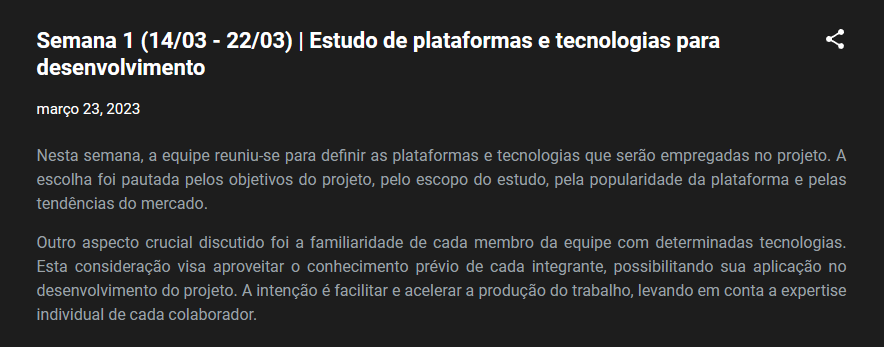
\includegraphics[scale=0.68]{./imagens/Blog1.png}
	\caption{Blog - Postagem 1}
    \label{fig:109}
\end{figure}

Na Figura \ref{fig:110} é apresentada a segunda postagem do blog.

\begin{figure}[H]
	\centering
	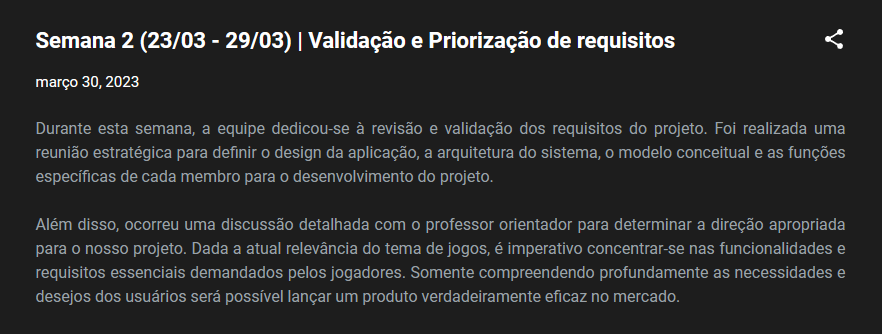
\includegraphics[scale=0.68]{./imagens/Blog2.png}
	\caption{Blog - Postagem 2}
    \label{fig:110}
\end{figure}
\pagebreak

Na Figura \ref{fig:111} é apresentada a terceira postagem do blog.

\begin{figure}[H]
	\centering
	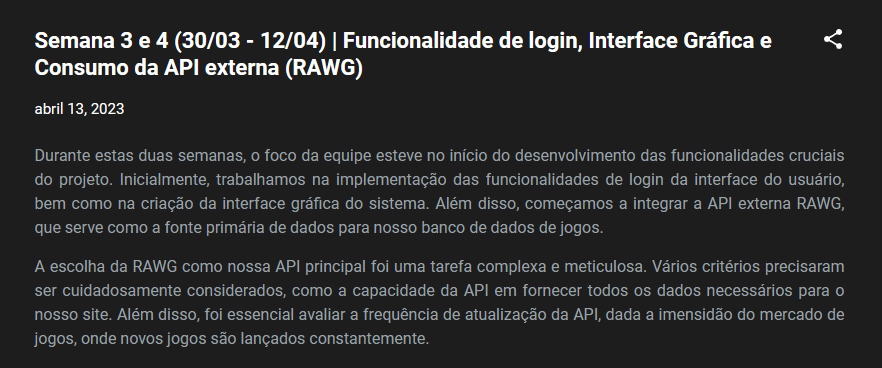
\includegraphics[scale=0.68]{./imagens/Blog3.png}
	\caption{Blog - Postagem 3}
    \label{fig:111}
\end{figure}

Na Figura \ref{fig:112} é apresentada a quarta postagem do blog.

\begin{figure}[H]
	\centering
	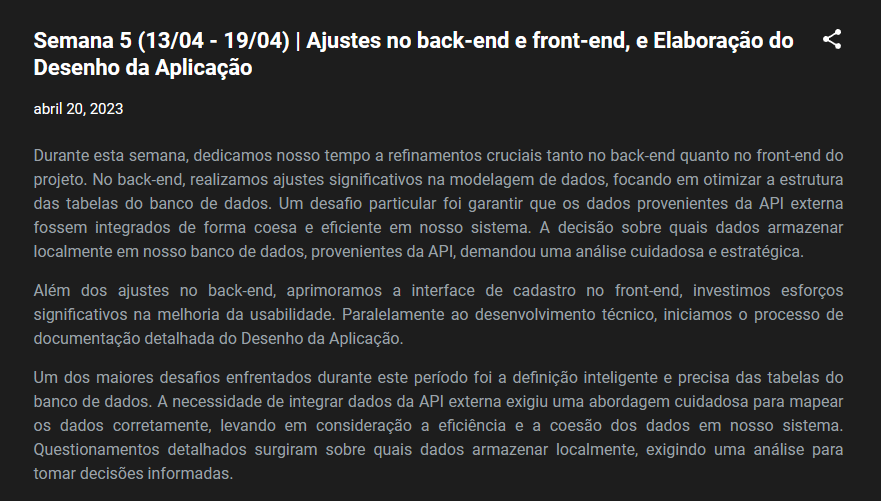
\includegraphics[scale=0.68]{./imagens/Blog4.png}
	\caption{Blog - Postagem 4}
    \label{fig:112}
\end{figure}
\pagebreak

Na Figura \ref{fig:113} é apresentada a quinta postagem do blog.

\begin{figure}[H]
	\centering
	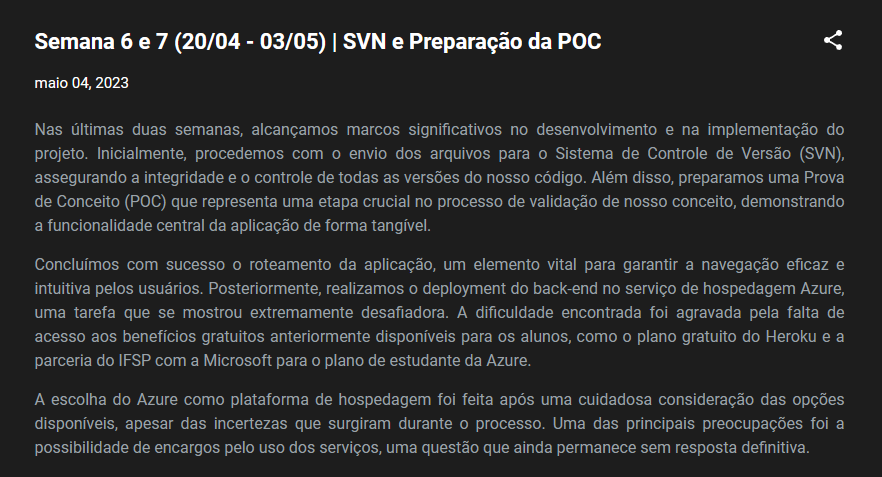
\includegraphics[scale=0.68]{./imagens/Blog5.png}
	\caption{Blog - Postagem 5}
    \label{fig:113}
\end{figure}

Na Figura \ref{fig:114} é apresentada a sexta postagem do blog.

\begin{figure}[H]
	\centering
	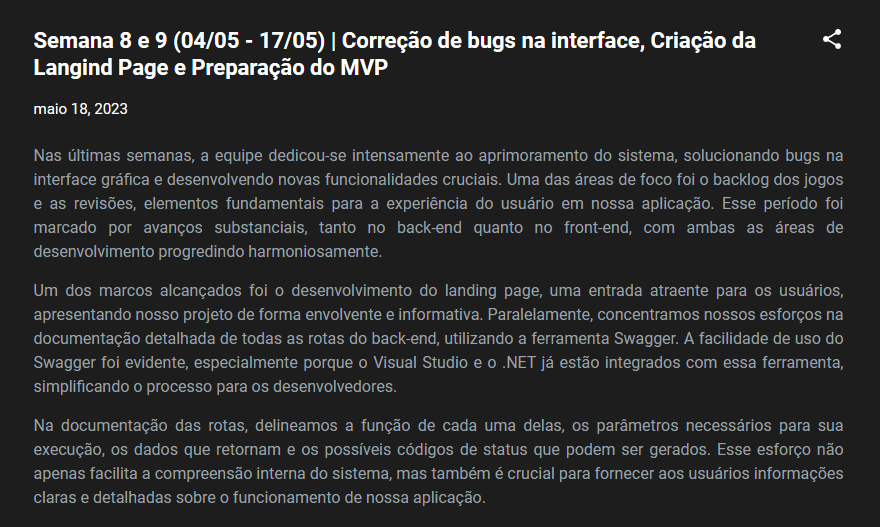
\includegraphics[scale=0.68]{./imagens/Blog6.png}
	\caption{Blog - Postagem 6}
    \label{fig:114}
\end{figure}
\pagebreak

Na Figura \ref{fig:115} é apresentada a sétima postagem do blog.

\begin{figure}[H]
	\centering
	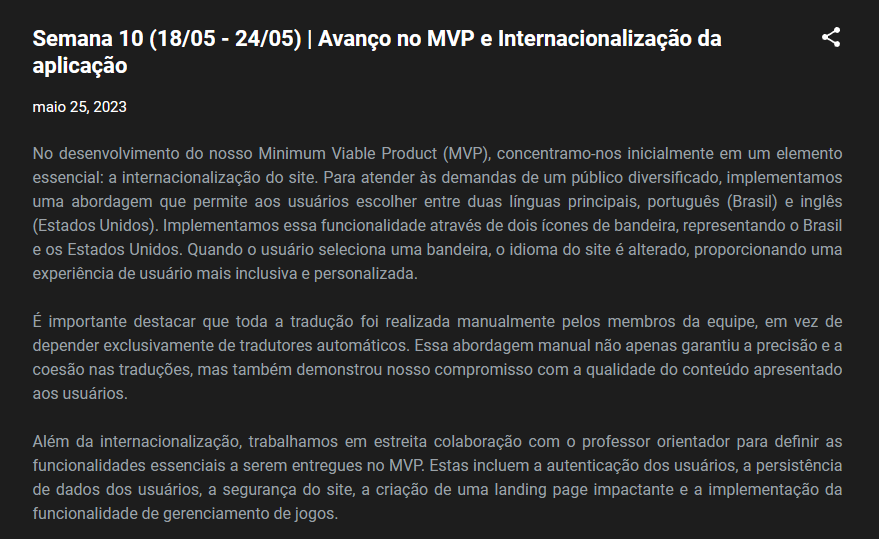
\includegraphics[scale=0.68]{./imagens/Blog7.png}
	\caption{Blog - Postagem 7}
    \label{fig:115}
\end{figure}
\pagebreak

Na Figura \ref{fig:116} é apresentada a oitava postagem do blog.

\begin{figure}[H]
	\centering
	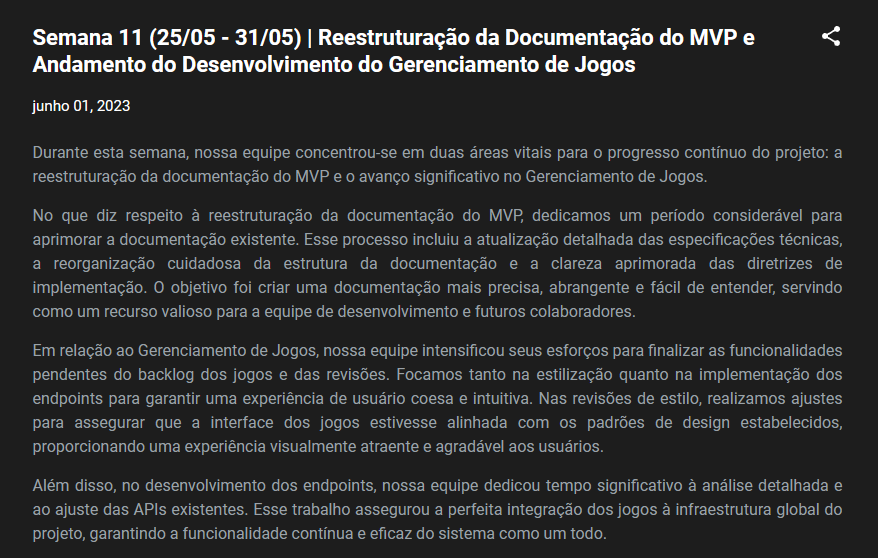
\includegraphics[scale=0.68]{./imagens/Blog8.png}
	\caption{Blog - Postagem 8}
    \label{fig:116}
\end{figure}
\pagebreak

Na Figura \ref{fig:117} é apresentada a nona postagem do blog.

\begin{figure}[H]
	\centering
	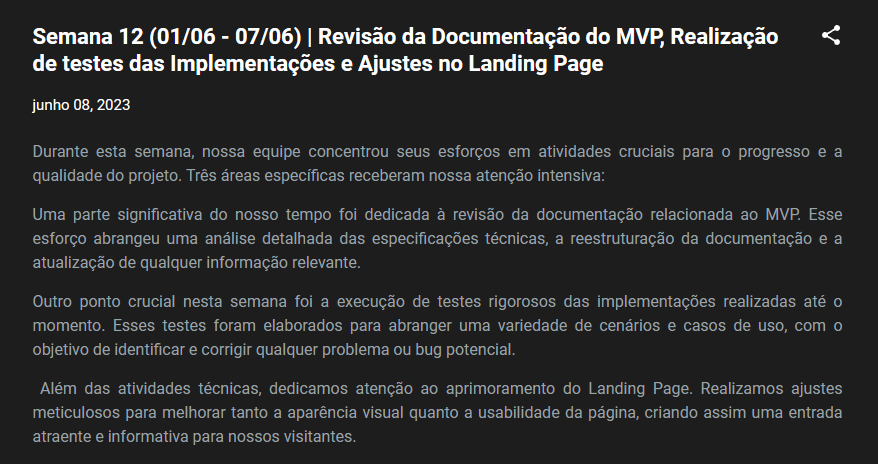
\includegraphics[scale=0.68]{./imagens/Blog9.png}
	\caption{Blog - Postagem 9}
    \label{fig:117}
\end{figure}

Na Figura \ref{fig:118} é apresentada a décima postagem do blog.

\begin{figure}[H]
	\centering
	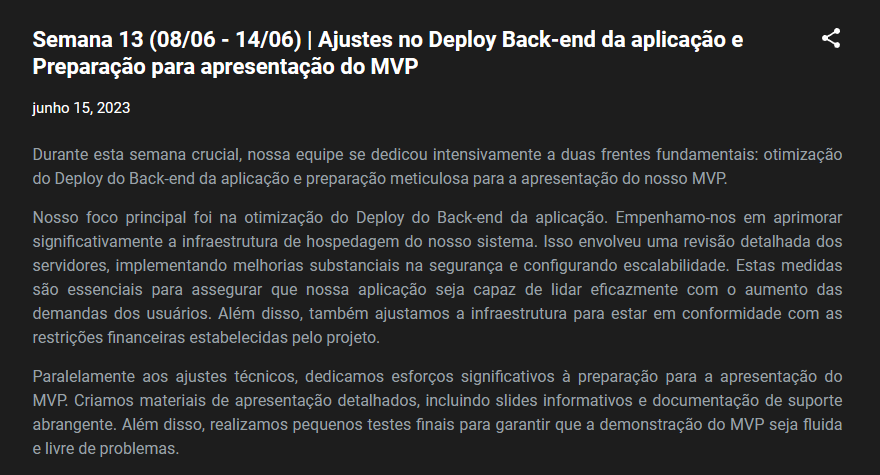
\includegraphics[scale=0.68]{./imagens/Blog10.png}
	\caption{Blog - Postagem 10}
    \label{fig:118}
\end{figure}
\pagebreak

Na Figura \ref{fig:119} é apresentada a undécima postagem do blog.

\begin{figure}[H]
	\centering
	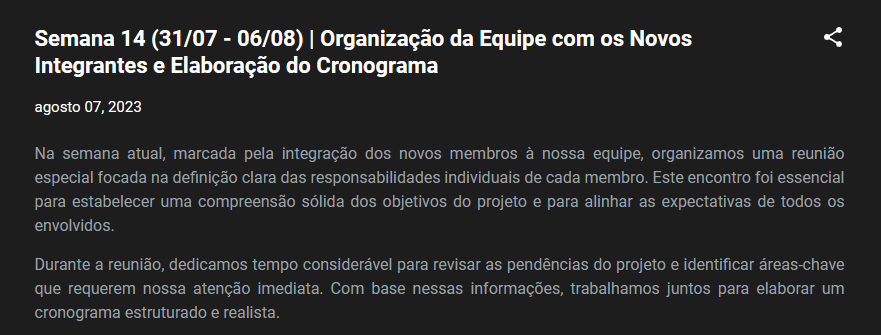
\includegraphics[scale=0.68]{./imagens/Blog11.png}
	\caption{Blog - Postagem 11}
    \label{fig:119}
\end{figure}

Na Figura \ref{fig:120} é apresentada a duodécima postagem do blog.

\begin{figure}[H]
	\centering
	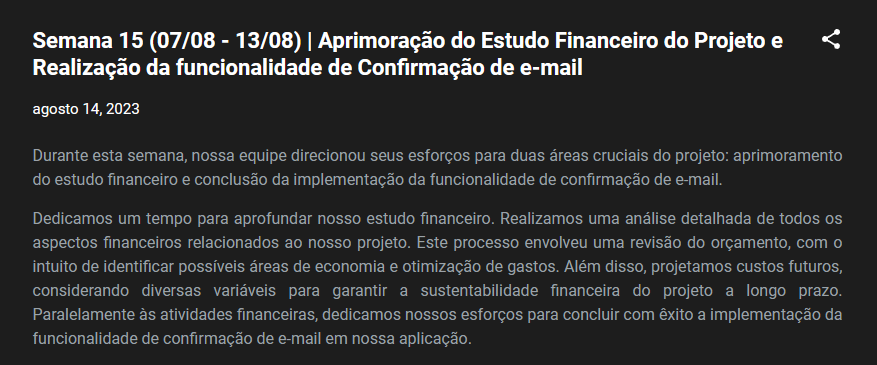
\includegraphics[scale=0.68]{./imagens/Blog12.png}
	\caption{Blog - Postagem 12}
    \label{fig:120}
\end{figure}
\pagebreak

Na Figura \ref{fig:121} é apresentada a décima terceira postagem do blog.

\begin{figure}[H]
	\centering
	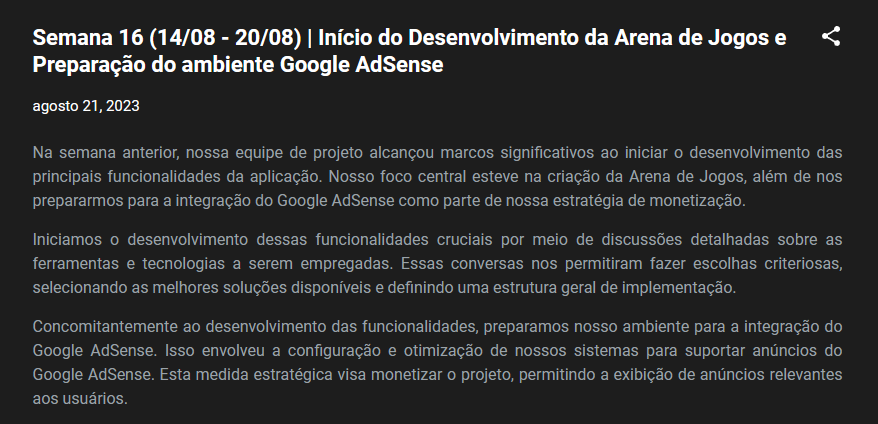
\includegraphics[scale=0.68]{./imagens/Blog13.png}
	\caption{Blog - Postagem 13}
    \label{fig:121}
\end{figure}

Na Figura \ref{fig:122} é apresentada a décima quarta postagem do blog.

\begin{figure}[H]
	\centering
	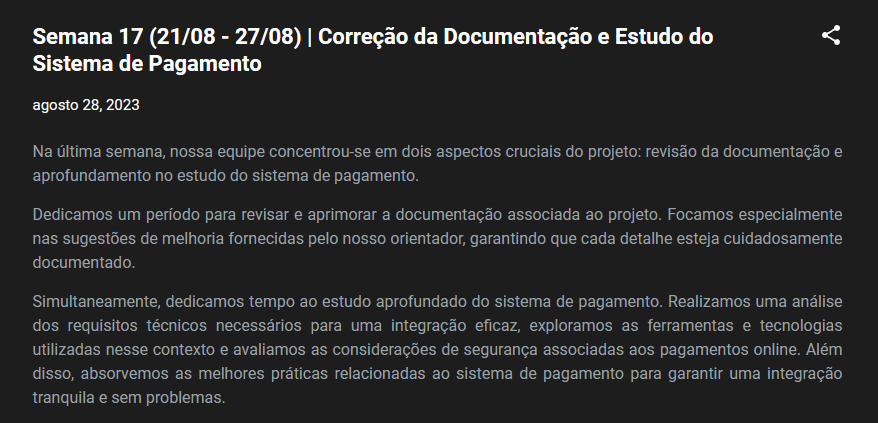
\includegraphics[scale=0.68]{./imagens/Blog14.png}
	\caption{Blog - Postagem 14}
    \label{fig:122}
\end{figure}
\pagebreak

Na Figura \ref{fig:123} é apresentada a décima quinta postagem do blog.

\begin{figure}[H]
	\centering
	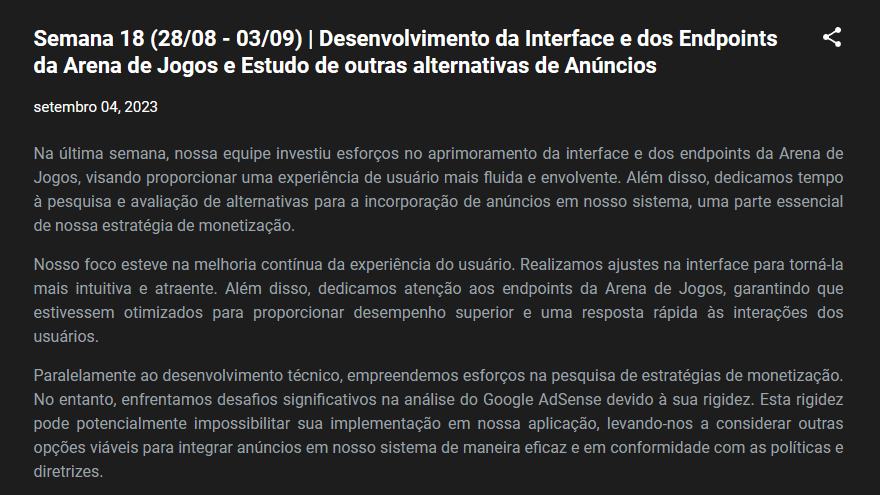
\includegraphics[scale=0.68]{./imagens/Blog15.png}
	\caption{Blog - Postagem 15}
    \label{fig:123}
\end{figure}

Na Figura \ref{fig:124} é apresentada a décima sexta postagem do blog.

\begin{figure}[H]
	\centering
	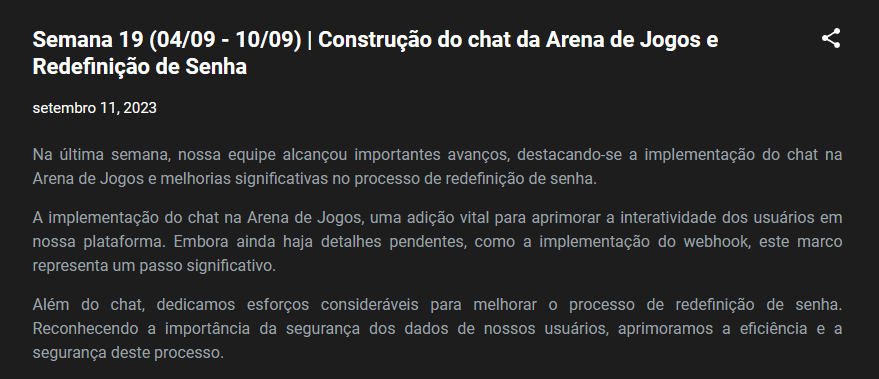
\includegraphics[scale=0.68]{./imagens/Blog16.png}
	\caption{Blog - Postagem 16}
    \label{fig:124}
\end{figure}
\pagebreak

Na Figura \ref{fig:125} é apresentada a décima sétima postagem do blog.

\begin{figure}[H]
	\centering
	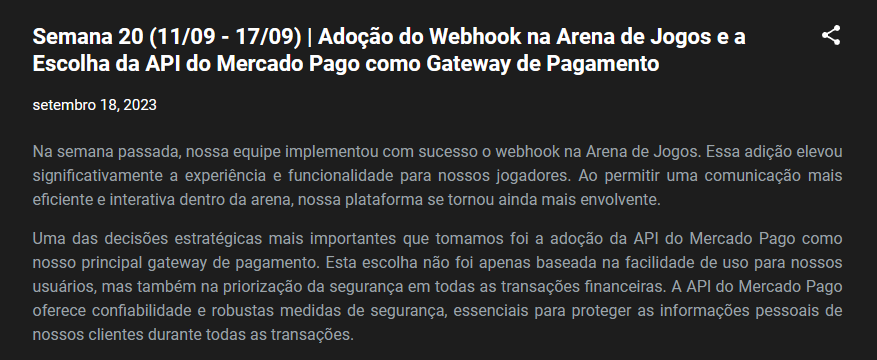
\includegraphics[scale=0.68]{./imagens/Blog17.png}
	\caption{Blog - Postagem 17}
    \label{fig:125}
\end{figure}

Na Figura \ref{fig:126} é apresentada a décima oitava postagem do blog.

\begin{figure}[H]
	\centering
	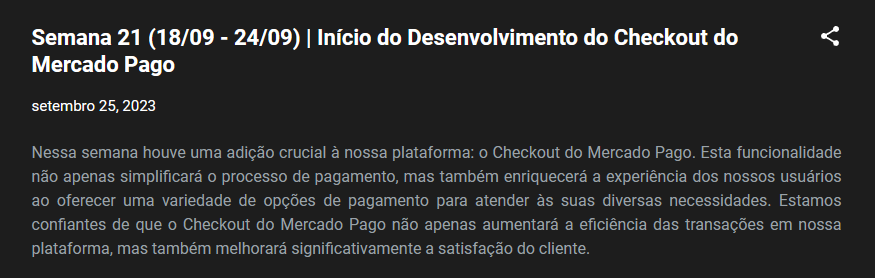
\includegraphics[scale=0.68]{./imagens/Blog18.png}
	\caption{Blog - Postagem 18}
    \label{fig:126}
\end{figure}
\pagebreak

Na Figura \ref{fig:127} é apresentada a décima nona postagem do blog.

\begin{figure}[H]
	\centering
	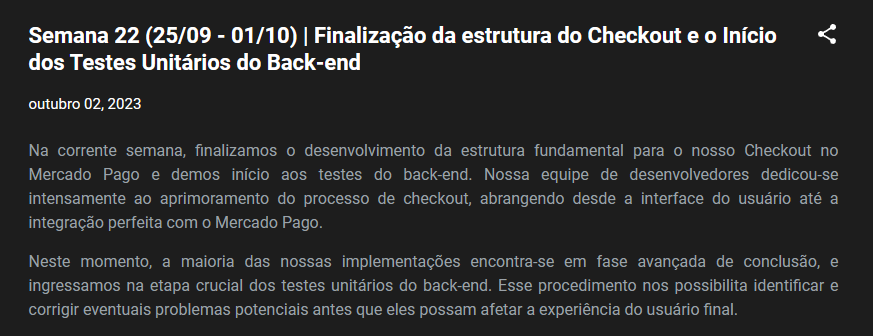
\includegraphics[scale=0.68]{./imagens/Blog19.png}
	\caption{Blog - Postagem 19}
    \label{fig:127}
\end{figure}

Na Figura \ref{fig:128} é apresentada a vigésima postagem do blog.

\begin{figure}[H]
	\centering
	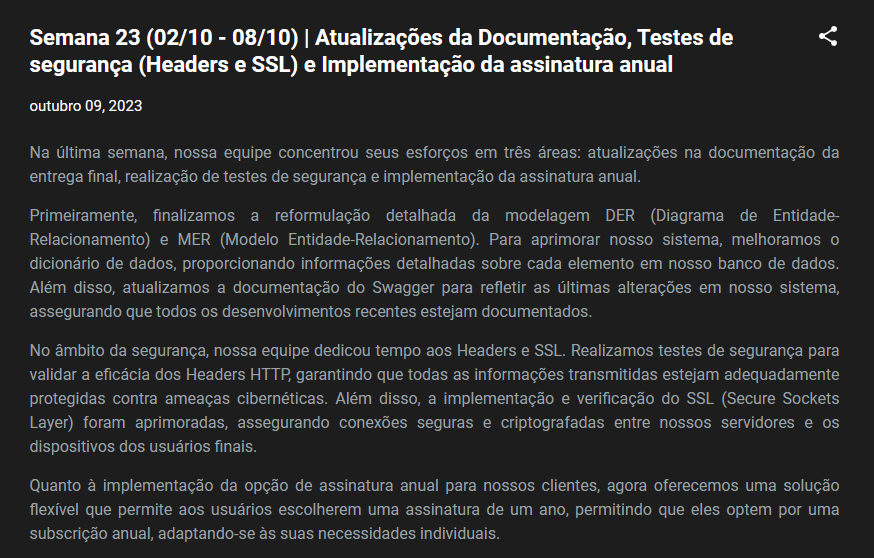
\includegraphics[scale=0.68]{./imagens/Blog20.png}
	\caption{Blog - Postagem 20}
    \label{fig:128}
\end{figure}
\pagebreak

Na Figura \ref{fig:129} é apresentada a vigésima primeira postagem do blog.

\begin{figure}[H]
	\centering
	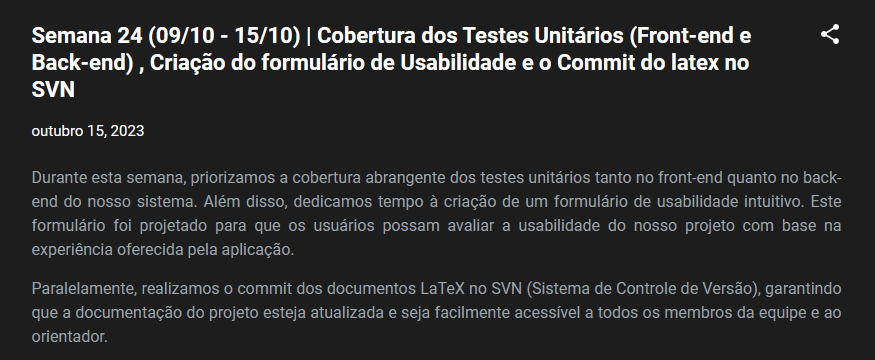
\includegraphics[scale=0.68]{./imagens/Blog21.png}
	\caption{Blog - Postagem 21}
    \label{fig:129}
\end{figure}


Na Figura \ref{fig:130} é apresentada a vigésima segunda postagem do blog.

\begin{figure}[H]
	\centering
	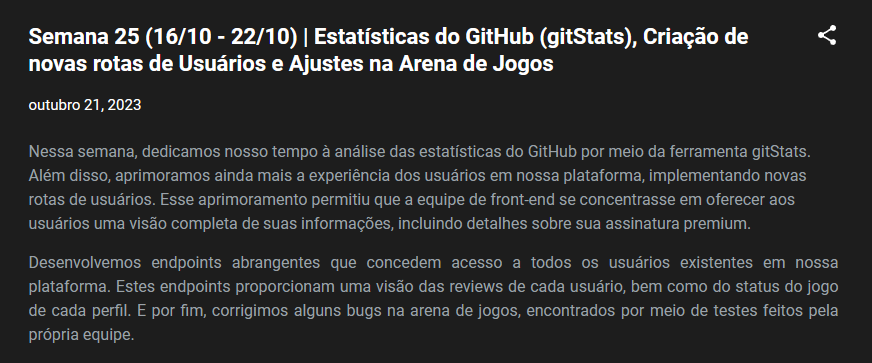
\includegraphics[scale=0.68]{./imagens/Blog22.png}
	\caption{Blog - Postagem 22}
    \label{fig:130}
\end{figure}
\pagebreak

Na Figura \ref{fig:131} é apresentada a vigésima terceira postagem do blog.

\begin{figure}[H]
	\centering
	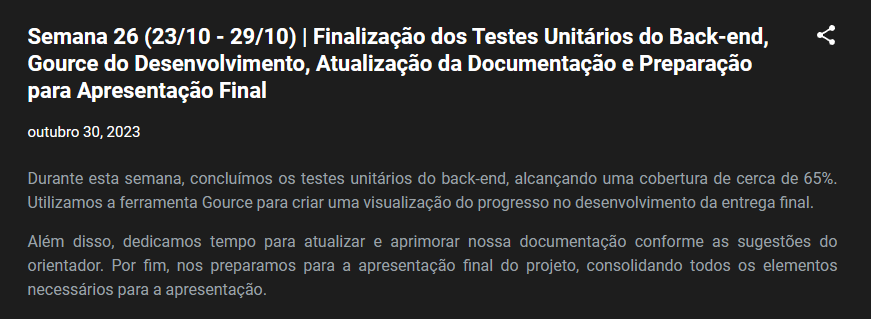
\includegraphics[scale=0.68]{./imagens/Blog23.png}
	\caption{Blog - Postagem 23}
    \label{fig:131}
\end{figure}

\chapter{Dicionário de Dados}
\label{DicionarioDados}

\begin{quadro}[h!]
\centering
\caption{AspNetUsers}
\label{tab:aspnetusers}
\begin{longtable}{|p{4cm}|p{2cm}|p{3cm}|p{5cm}|}
\hline
Campo & Chave & Tipo & Descrição
\\\hline
Id & PK & int & Identificador de um usuário
\\\hline
Phone & - & nvarchar(MAX) & Número de telefone do usuário
\\\hline
BirthDate & - & datetime & Data de nascimento do usuário
\\\hline
FirstName & - & nvarchar(MAX) & Primeiro nome do usuário
\\\hline
LastName & - & nvarchar(MAX) & Sobrenome do usuário
\\\hline
Email & - & nvarchar(256) & E-mail do usuário
\\\hline
UserName & - & nvarchar(256) & Nome de usuário
\\\hline
NormalizedUserName & - & nvarchar(256) & Sobrenome do usuário normalizado
\\\hline
NormalizedEmail & - & nvarchar(256) & E-mail do usuário normalizado
\\\hline
EmailConfirmed & - & bit & Controle para checar se o e-mail do usuário foi confirmado
\\\hline
PasswordHash & - & nvarchar(MAX) & Hash da senha
\\\hline
SecurityStamp & - & nvarchar(MAX) & Estado atual do usuário
\\\hline
ConcurrencyStamp & - & nvarchar(MAX) & Estado de criação do usuário
\\\hline
PhoneNumber & - & nvarchar(MAX) & Número de telefone do usuário
\\\hline
\end{longtable}
\fonte{Os Autores.}
\end{quadro}

\begin{quadro}[h!]
\centering
\caption{GameGenres}
\label{tab:gamegenres}
\begin{longtable}{|p{4cm}|p{2cm}|p{3cm}|p{5cm}|}
\hline
Campo & Chave & Tipo & Descrição
\\\hline
GameId & PK & int & Identificador composto para o Game
\\\hline
GenreId & PK & int & Identificador composto para o Genre
\\\hline
\end{longtable}
\fonte{Os Autores.}
\end{quadro}

\begin{quadro}[h!]
\centering
\caption{GamePlatforms}
\label{tab:gameplatforms}
\begin{longtable}{|p{4cm}|p{2cm}|p{3cm}|p{5cm}|}
\hline
Campo & Chave & Tipo & Descrição
\\\hline
GameId & PK & int & Identificador composto para o Game
\\\hline
PlatformId & PK & int & Identificador composto para a Platform
\\\hline
\end{longtable}
\fonte{Os Autores.}
\end{quadro}

\begin{quadro}[h!]
\centering
\caption{Games}
\label{tab:games}
\begin{longtable}{|p{4cm}|p{2cm}|p{3cm}|p{5cm}|}
\hline
Campo & Chave & Tipo & Descrição
\\\hline
Id & PK & int & Identificador para o jogo
\\\hline
ApiId & - & int & Identificador para o jogo na api externa
\\\hline
Name & - & nvarchar(MAX) & Nome do jogo
\\\hline
UrlImage & - & nvarchar(MAX) & Url da imagem do jogo
\\\hline
Metacritic & - & float & Nota do jogo no site Metacritic
\\\hline
ReleaseDate & - & datetime & Data de lançamento do jogo
\\\hline
\end{longtable}
\fonte{Os Autores.}
\end{quadro}

\begin{quadro}[h!]
\centering
\caption{Genres}
\label{tab:genres}
\begin{longtable}{|p{4cm}|p{2cm}|p{3cm}|p{5cm}|}
\hline
Campo & Chave & Tipo & Descrição
\\\hline
Id & PK & int & Identificador do gênero
\\\hline
EGenre & - & nvarchar(MAX) & Valor do gênero
\\\hline
\end{longtable}
\fonte{Os Autores.}
\end{quadro}

\begin{quadro}[h!]
\centering
\caption{Platforms}
\label{tab:platforms}
\begin{longtable}{|p{4cm}|p{2cm}|p{3cm}|p{5cm}|}
\hline
Campo & Chave & Tipo & Descrição
\\\hline
Id & PK & int & Identificador da plataforma
\\\hline
EPlatform & - & nvarchar(MAX) & Valor da plataforma
\\\hline
\end{longtable}
\fonte{Os Autores.}
\end{quadro}

\begin{quadro}[h!]
\centering
\caption{Reviews}
\label{tab:reviews}
\begin{longtable}{|p{4cm}|p{2cm}|p{3cm}|p{5cm}|}
\hline
Campo & Chave & Tipo & Descrição
\\\hline
Id & PK & int & Identificador da review
\\\hline
GameId & FK & int & Identificador do jogo presente na review
\\\hline
UserId & FK & int & Identificador do usuário responsável pela review
\\\hline
Score & - & int & Nota da review
\\\hline
Comment & - & nvarchar(MAX) & Comentário sobre o jogo
\\\hline
ReviewDate & - & datetime & Data de criação da review
\\\hline
GameStatus & - & int & Status do jogo
\\\hline
Favorite & - & bit & Controle para checar se o jogo está favoritado ou não
\\\hline
\end{longtable}
\fonte{Os Autores.}
\end{quadro}

\begin{quadro}[h!]
\centering
\caption{Subscriptions}
\label{tab:subscriptions}
\begin{longtable}{|p{4cm}|p{2cm}|p{3cm}|p{5cm}|}
\hline
Campo & Chave & Tipo & Descrição
\\\hline
Id & PK & int & Identificador da assinatura
\\\hline
IdPayer & - & int & Identificador do pagador da assinatura, na API do Mercado Pago
\\\hline
IdPlan & - & int & Identificador do plano, na API do Mercado Pago
\\\hline
StartDate & - & datetime & Data de Início da assinatura
\\\hline
LastPaymentDate & - & datetime & Data do último pagamento
\\\hline
IsActive & - & bit & Controle que indica se a assinatura está ativa
\\\hline
CancelDate & - & datetime & Data de cancelamento da assinatura, se houver
\\\hline
SubscriptionType & - & nvarchar(50) & Indica o tipo de assinatura (mensal ou anual)
\\\hline
UserId & FK & nvarchar(50) &Identificador do usuário ao qual a assinatura pertence
\\\hline
SubscriptionMPId & - & nvarchar(50) &Identificador da assinatura, na API do Mercado Pago
\\\hline
\end{longtable}
\fonte{Os Autores.}
\end{quadro}

\begin{quadro}[h!]
\centering
\caption{Payments}
\label{tab:payments}
\begin{longtable}{|p{4cm}|p{2cm}|p{3cm}|p{5cm}|}
\hline
Campo & Chave & Tipo & Descrição
\\\hline
Id & PK & int & Identificador do pagamento
\\\hline
PaymentDate & - & datetime & Data do pagamento
\\\hline
IdPayment & - & int & Identificador do pagamento, na API do Mercado Pago
\\\hline
SubscriptionId & FK & int & Identificador da assinatura
\\\hline
IdSubscription & - & int & Identificador da assinatura, na API do Mercado Pago
\\\hline
\end{longtable}
\fonte{Os Autores.}
\end{quadro}

\chapter{Métricas}
\label{Métricas}

Este apêndice apresenta as estatísticas relacionadas aos repositórios do projeto no GitHub, utilizando a ferramenta gitStats.

Na Figura \ref{generalFrontend} são apresentados os dados gerais do repositório GitHub referentes ao front-end.

\begin{figure}[H]
	\centering
	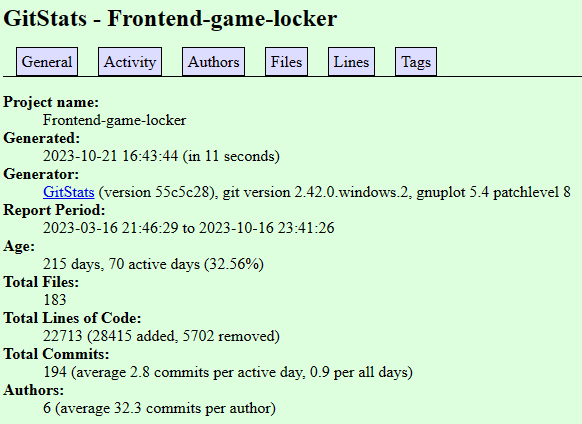
\includegraphics[scale=0.8]{./imagens/metricas/gitStatsFrontend/gitStatsGeneral.png}
	\caption{Dados Gerais do Repositório Front-end}
	Fonte: Os autores
    \label{generalFrontend}
\end{figure}
\pagebreak

Na Figura \ref{weeklyActivityFrontend} são apresentadas as estatísticas de atividade semanal do repositório GitHub referentes ao \textit{front-end}.

\begin{figure}[H]
	\centering
	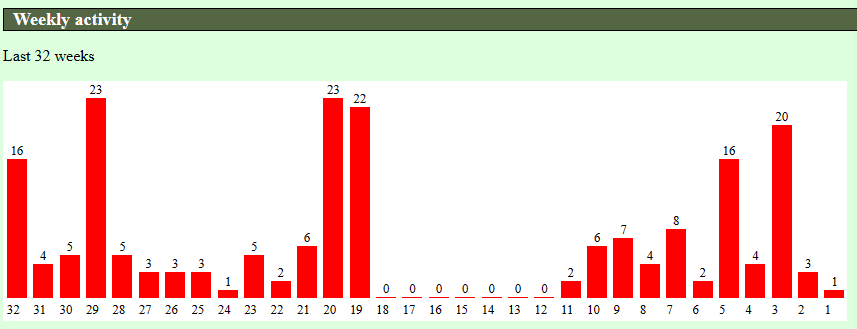
\includegraphics[scale=0.7]{./imagens/metricas/gitStatsFrontend/activity/weeklyActivity.png}
	\caption{Atividade semanal do Repositório Front-end}
	Fonte: Os autores
    \label{weeklyActivityFrontend}
\end{figure}

Na Figura \ref{hourOfDayFrontend}, são apresentadas as estatísticas de \textit{commits} por hora do dia do repositório GitHub relacionadas ao \textit{front-end}.

\begin{figure}[H]
	\centering
	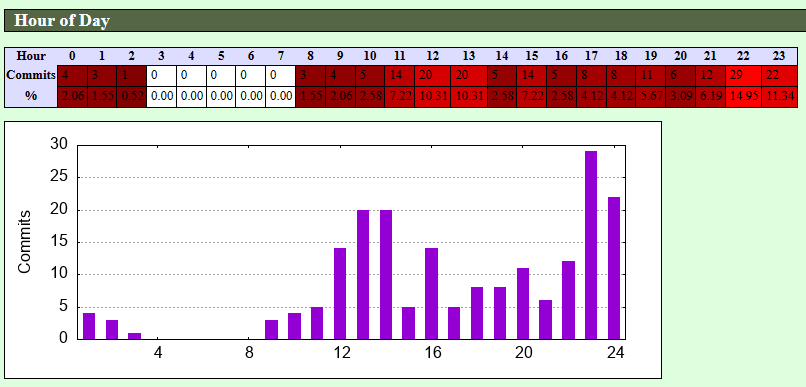
\includegraphics[scale=0.7]{./imagens/metricas/gitStatsFrontend/activity/hourOfDay.png}
	\caption{\textit{Commits} por hora do dia do Repositório Front-end}
	Fonte: Os autores
    \label{hourOfDayFrontend}
\end{figure}
\pagebreak

Na Figura \ref{hourOfWeekFrontend}, são apresentadas as estatísticas de \textit{commits} por hora da semana do repositório GitHub relacionadas ao \textit{front-end}.

\begin{figure}[H]
	\centering
	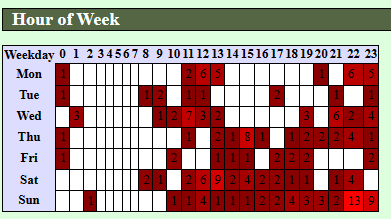
\includegraphics[scale=1]{./imagens/metricas/gitStatsFrontend/activity/hourOfWeek.png}
	\caption{\textit{Commits} por hora da semana do Repositório Front-end}
	Fonte: Os autores
    \label{hourOfWeekFrontend}
\end{figure}

Na Figura \ref{dayOfWeekFrontend}, são apresentadas as estatísticas de \textit{commits} por dia da semana do repositório GitHub relacionadas ao \textit{front-end}.

\begin{figure}[H]
	\centering
	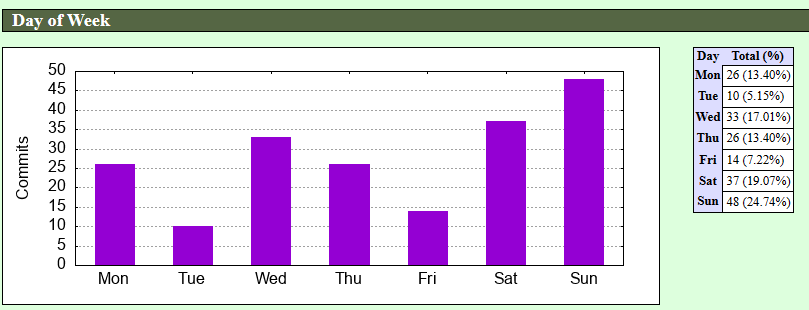
\includegraphics[scale=0.7]{./imagens/metricas/gitStatsFrontend/activity/dayOfWeek.png}
	\caption{\textit{Commits} por dia da semana do Repositório Front-end}
	Fonte: Os autores
    \label{dayOfWeekFrontend}
\end{figure}
\pagebreak

Na Figura \ref{monthOfYearFrontend}, são apresentadas as estatísticas de \textit{commits} por mês do ano do repositório GitHub relacionadas ao \textit{front-end}.

\begin{figure}[H]
	\centering
	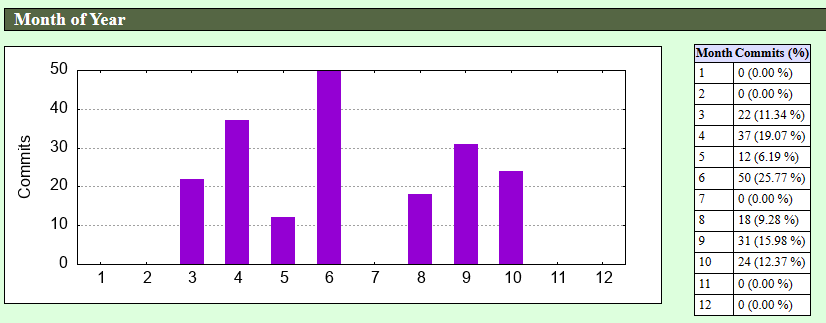
\includegraphics[scale=0.7]{./imagens/metricas/gitStatsFrontend/activity/monthOfYear.png}
	\caption{\textit{Commits} por mês do ano do Repositório Front-end}
	Fonte: Os autores
    \label{monthOfYearFrontend}
\end{figure}

Na Figura \ref{commitsFrontend}, são apresentadas as estatísticas de \textit{commits} por ano/mês do repositório GitHub relacionadas ao \textit{front-end}.

\begin{figure}[H]
	\centering
	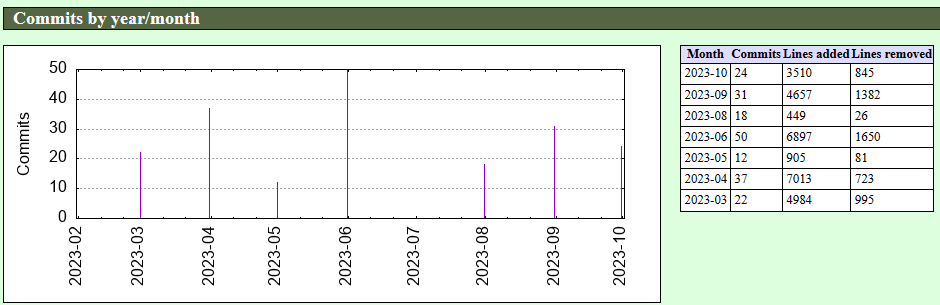
\includegraphics[scale=0.6]{./imagens/metricas/gitStatsFrontend/activity/commits.png}
	\caption{\textit{Commits} por ano/mês do Repositório Front-end}
	Fonte: Os autores
    \label{commitsFrontend}
\end{figure}
\pagebreak

Na Figura \ref{listOfAuthorsFrontend}, é apresentada a lista dos autores do repositório GitHub relacionadas ao \textit{front-end}.

\begin{figure}[H]
	\centering
	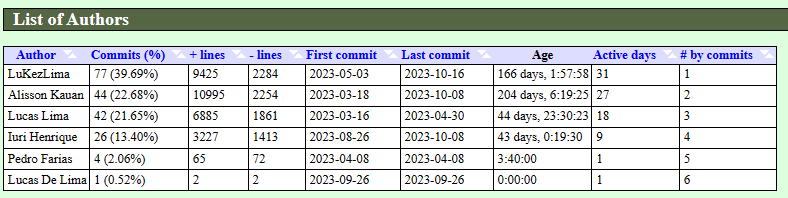
\includegraphics[scale=0.7]{./imagens/metricas/gitStatsFrontend/authors/listOfAuthors.png}
	\caption{Lista dos autores do Repositório Front-end}
	Fonte: Os autores
    \label{listOfAuthorsFrontend}
\end{figure}

Na Figura \ref{cumulatedLinesFrontend}, são apresentadas as linhas de código acumuladas do repositório GitHub relacionadas ao \textit{front-end}.

\begin{figure}[H]
	\centering
	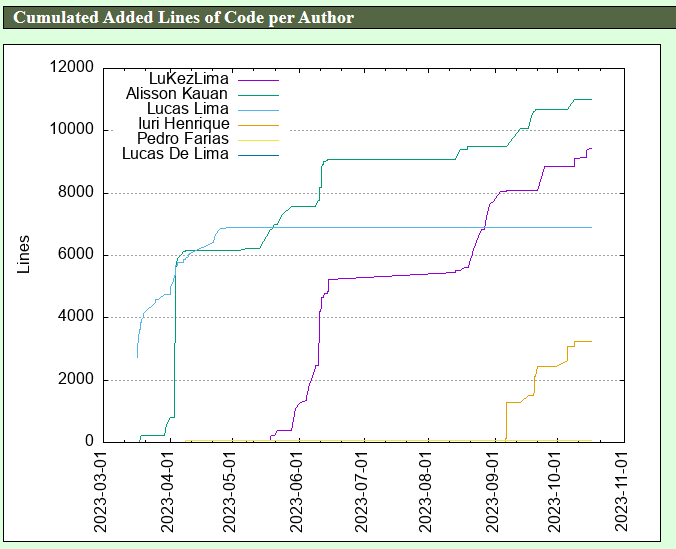
\includegraphics[scale=0.7]{./imagens/metricas/gitStatsFrontend/authors/cumulatedLines.png}
	\caption{Linhas de código acumuladas do Repositório Front-end}
	Fonte: Os autores
    \label{cumulatedLinesFrontend}
\end{figure}
\pagebreak

Na Figura \ref{commitPerAuthorFrontend}, são apresentadas as estatísticas de \textit{commits} por autor do repositório GitHub relacionadas ao \textit{front-end}.

\begin{figure}[H]
	\centering
	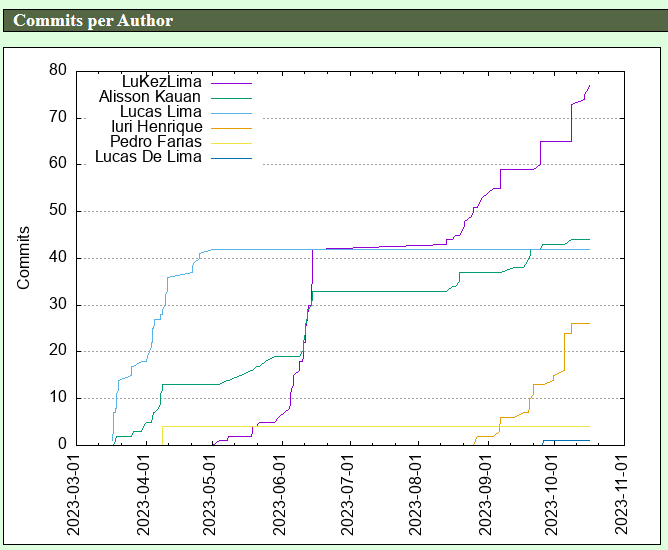
\includegraphics[scale=0.7]{./imagens/metricas/gitStatsFrontend/authors/commitPerAuthor.png}
	\caption{\textit{Commits} por autor do Repositório Front-end}
	Fonte: Os autores
    \label{commitPerAuthorFrontend}
\end{figure}

Na Figura \ref{filesFrontend}, são apresentados os dados de arquivos do repositório GitHub relacionadas ao \textit{front-end}.

\begin{figure}[H]
	\centering
	\includegraphics[scale=1]{./imagens/metricas/gitStatsFrontend/files/files.png}
	\caption{Dados de arquivo do Repositório Front-end}
	Fonte: Os autores
    \label{filesFrontend}
\end{figure}
\pagebreak

Na Figura \ref{fileCountFrontend}, são apresentadas as estatísticas de contagem de arquivo por data do repositório GitHub relacionadas ao \textit{front-end}.

\begin{figure}[H]
	\centering
	\includegraphics[scale=0.8]{./imagens/metricas/gitStatsFrontend/files/fileCount.png}
	\caption{Contagem de arquivo por data do Repositório Front-end}
	Fonte: Os autores
    \label{fileCountFrontend}
\end{figure}

Na Figura \ref{extensionsFrontend}, são apresentadas as estatísticas de extensões do repositório GitHub relacionadas ao \textit{front-end}.

\begin{figure}[H]
	\centering
	\includegraphics[scale=1]{./imagens/metricas/gitStatsFrontend/files/extensions.png}
	\caption{Extensões do Repositório Front-end}
	Fonte: Os autores
    \label{extensionsFrontend}
\end{figure}
\pagebreak

Na Figura \ref{linesFrontend}, são apresentadas as estatísticas de linhas de código do repositório GitHub relacionadas ao \textit{front-end}.

\begin{figure}[H]
	\centering
	\includegraphics[scale=0.8]{./imagens/metricas/gitStatsFrontend/lines/linesOfCode.png}
	\caption{Linhas de código do Repositório Front-end}
	Fonte: Os autores
    \label{linesFrontend}
\end{figure}

Na Figura \ref{generalBackend} são apresentados os dados gerais do repositório GitHub referentes ao \textit{back-end}.

\begin{figure}[H]
	\centering
	\includegraphics[scale=0.8]{./imagens/metricas/gitStatsBackend/gitStatsGeneral.png}
	\caption{Dados Gerais do Repositório Back-end}
	Fonte: Os autores
    \label{generalBackend}
\end{figure}
\pagebreak

Na Figura \ref{weeklyActivityBackend} são apresentadas as estatísticas de atividade semanal do repositório GitHub referentes ao \textit{back-end}.

\begin{figure}[H]
	\centering
	\includegraphics[scale=0.7]{./imagens/metricas/gitStatsBackend/activity/weeklyActivity.png}
	\caption{Atividade semanal do Repositório Back-end}
	Fonte: Os autores
    \label{weeklyActivityBackend}
\end{figure}

Na Figura \ref{hourOfDayBackend}, são apresentadas as estatísticas de \textit{commits} por hora do dia do repositório GitHub relacionadas ao \textit{back-end}.

\begin{figure}[H]
	\centering
	\includegraphics[scale=0.7]{./imagens/metricas/gitStatsBackend/activity/hourOfDay.png}
	\caption{\textit{Commits} por hora do dia do Repositório Back-end}
	Fonte: Os autores
    \label{hourOfDayBackend}
\end{figure}
\pagebreak

Na Figura \ref{hourOfWeekBackend}, são apresentadas as estatísticas de \textit{commits} por hora da semana do repositório GitHub relacionadas ao \textit{back-end}.

\begin{figure}[H]
	\centering
	\includegraphics[scale=1]{./imagens/metricas/gitStatsBackend/activity/hourOfWeek.png}
	\caption{\textit{Commits} por hora da semana do Repositório Back-end}
	Fonte: Os autores
    \label{hourOfWeekBackend}
\end{figure}

Na Figura \ref{dayOfWeekBackend}, são apresentadas as estatísticas de \textit{commits} por dia da semana do repositório GitHub relacionadas ao \textit{back-end}.

\begin{figure}[H]
	\centering
	\includegraphics[scale=0.7]{./imagens/metricas/gitStatsBackend/activity/dayOfWeek.png}
	\caption{\textit{Commits} por dia da semana do Repositório Back-end}
	Fonte: Os autores
    \label{dayOfWeekBackend}
\end{figure}
\pagebreak

Na Figura \ref{monthOfYearBackend}, são apresentadas as estatísticas de \textit{commits} por mês do ano do repositório GitHub relacionadas ao \textit{back-end}.

\begin{figure}[H]
	\centering
	\includegraphics[scale=0.7]{./imagens/metricas/gitStatsBackend/activity/monthOfYear.png}
	\caption{\textit{Commits} por mês do ano do Repositório Back-end}
	Fonte: Os autores
    \label{monthOfYearBackend}
\end{figure}

Na Figura \ref{commitsBackend}, são apresentadas as estatísticas de \textit{commits} por ano/mês do repositório GitHub relacionadas ao \textit{back-end}.

\begin{figure}[H]
	\centering
	\includegraphics[scale=0.6]{./imagens/metricas/gitStatsBackend/activity/commits.png}
	\caption{\textit{Commits} por ano/mês do Repositório Back-end}
	Fonte: Os autores
    \label{commitsBackend}
\end{figure}
\pagebreak

Na Figura \ref{listOfAuthorsBackend}, é apresentada a lista dos autores do repositório GitHub relacionadas ao \textit{back-end}.

\begin{figure}[H]
	\centering
	\includegraphics[scale=0.65]{./imagens/metricas/gitStatsBackend/authors/listOfAuthors.png}
	\caption{Lista dos autores do Repositório Back-end}
	Fonte: Os autores
    \label{listOfAuthorsBackend}
\end{figure}

Na Figura \ref{cumulatedLinesBackend}, são apresentadas as linhas de código acumuladas do repositório GitHub relacionadas ao \textit{back-end}.

\begin{figure}[H]
	\centering
	\includegraphics[scale=0.7]{./imagens/metricas/gitStatsBackend/authors/cumulatedLines.png}
	\caption{Linhas de código acumuladas do Repositório Back-end}
	Fonte: Os autores
    \label{cumulatedLinesBackend}
\end{figure}
\pagebreak

Na Figura \ref{commitPerAuthorBackend}, são apresentadas as estatísticas de \textit{commits} por autor do repositório GitHub relacionadas ao \textit{back-end}.

\begin{figure}[H]
	\centering
	\includegraphics[scale=0.7]{./imagens/metricas/gitStatsBackend/authors/commitsPerAuthors.png}
	\caption{\textit{Commits} por autor do Repositório Back-end}
	Fonte: Os autores
    \label{commitPerAuthorBackend}
\end{figure}

Na Figura \ref{filesBackend}, são apresentados os dados de arquivos do repositório GitHub relacionadas ao \textit{back-end}.

\begin{figure}[H]
	\centering
	\includegraphics[scale=1]{./imagens/metricas/gitStatsBackend/files/files.png}
	\caption{Dados de arquivo do Repositório Back-end}
	Fonte: Os autores
    \label{filesBackend}
\end{figure}
\pagebreak

Na Figura \ref{fileCountBackend}, são apresentadas as estatísticas de contagem de arquivo por data do repositório GitHub relacionadas ao \textit{back-end}.

\begin{figure}[H]
	\centering
	\includegraphics[scale=0.8]{./imagens/metricas/gitStatsBackend/files/fileCount.png}
	\caption{Contagem de arquivo por data do Repositório Back-end}
	Fonte: Os autores
    \label{fileCountBackend}
\end{figure}

Na Figura \ref{extensionsBackend}, são apresentadas as estatísticas de extensões do repositório GitHub relacionadas ao \textit{back-end}.

\begin{figure}[H]
	\centering
	\includegraphics[scale=1]{./imagens/metricas/gitStatsBackend/files/extensions.png}
	\caption{Extensões do Repositório Back-end}
	Fonte: Os autores
    \label{extensionsBackend}
\end{figure}
\pagebreak

Na Figura \ref{linesBackend}, são apresentadas as estatísticas de linhas de código do repositório GitHub relacionadas ao \textit{back-end}.

\begin{figure}[H]
	\centering
	\includegraphics[scale=0.8]{./imagens/metricas/gitStatsBackend/lines/linesOfCode.png}
	\caption{Linhas de código do Repositório Back-end}
	Fonte: Os autores
    \label{linesBackend}
\end{figure}

\chapter{Termos e Condições}
\label{termos-e-condicoes}
\index{pdf}
\includepdf[pages= - ,scale=0.8,frame=true,pagecommand={}]{documentos/Termos_e_Condições.pdf}

\end{apendicesenv}
% ---
